% -----------------------------------------------------------------------------
\section{SBOL Data Model}\label{sec:model}
% -----------------------------------------------------------------------------

In this section, we describe the types of biological design data that can belong to an SBOL document and the relationships between these data types. The SBOL data model is specified using Unified Modeling Language (UML) 2.0 diagrams \href{http://www.omg.org/spec/UML/2.0/}{(OMG 2005)}. Subsections \ref{sec:umldiagrams}, \ref{sec:nameconventions}, \ref{sec:datatypes} review the basics of UML diagrams and explain the naming conventions and generic data types used in this specification. The remaining sections then describe the SBOL data model in detail. Complete SBOL examples and best practices when using the standard can be found in \ref{sec:examples} and \ref{sec:bestpractices}, respectively. 

\subsection{Understanding the UML Diagrams}
\label{sec:umldiagrams}

The types of biological design data modeled by SBOL are commonly referred to as {\em classes}, especially when discussing the details of software implementation. Each SBOL class can be instantiated by many SBOL objects. These objects may contain data that differ in content, but they MUST agree on the type and form of their data as dictated by their common class. Classes are represented in UML diagrams as rectangles labeled at the top with class names.

Classes may be connected to other classes by association properties, which are represented in UML diagrams as arrows. These arrows are labeled with data cardinalities in order to indicate how many values a given association property may possess (see below). The remaining (non-association) properties of a class are listed below its name. Each of the latter properties is labeled with its data type and cardinality.

In the case of an association property, the class from which the arrow originates is the owner of the association property. A diamond at the origin of the arrow indicates the type of association. Open-faced diamonds indicate shared aggregation, in which the owner of the association property exists independently of its value. In the SBOL data model, the value of an association property MUST be a URI or set of URIs that refer to SBOL objects belonging to the class at the tip of the arrow.

By contrast, filled diamonds indicate composite aggregation, also known as a part-whole relationship, in which the value of the association property MUST NOT exist independently of its owner. In addition, in the SBOL data model, it is REQUIRED that the value of each composite aggregation property is a unique SBOL object (that is, not the value for more than one such property).
%For example, it will later be shown how objects of the \sbol{SequenceAnnotation} class must associated with an object of the \sbol{ComponentDefinition} class (and only that object).

All SBOL properties are labeled with one of several restrictions on data cardinality. These are:

\begin{itemize}

\item $1$ - required, one: there must be exactly one value for this property.

\item $0 \ldots 1$ - optional: there may be a single value for this property or it may be absent.

\item $0 \ldots *$ - unbounded: there may be any number of values for this property, including none.

\item $1 \ldots *$ - required, unbounded: there may be any number of values for this property, as long as there is at least one.

\item $n \ldots *$ - at least: there must be at least $n$ values for this property.

\end{itemize}

Finally, classes can inherit the properties of other classes. Inheritance relationships are represented in UML diagrams as open-faced, triangular arrows that point from the inheriting class to the inherited class. Some classes in the SBOL data model cannot be instantiated as objects and exist only to group common properties for inheritance. These classes have italicized names and are known as abstract classes.

\subsection{Naming and Font Conventions}
\label{sec:nameconventions}

SBOL classes are named using upper "camel case," meaning that each word is capitalized and all words are run together without spaces e.g. \sbol{Identified}, \sbol{SequenceAnnotation}.  
Properties, on the other hand, are named using lower camel case, meaning that they begin lower case (e.g., \sbol{identity}) but if they consist of multiple words, all words after the first begin with an upper case letter (e.g., \sbol{persistentIdentity}).

Within the SBOL data model, each property is given a singular or plural name in accordance with its data cardinalities. The forms of these names follow the usual rules of grammar. For example, \sbol{SequenceAnnotation} is the singular form of \sbol{SequenceAnnotation}s. 

When SBOL objects are serialized to be exchanged (using \emph{Resource Description Framework} (RDF) as described in \ref{sec:serialization}), however, SBOL properties are always given singular names. This is because the SBOL data model does not contain classes that correspond directly to the RDF elements that group other elements into ordered or unordered sets. Consequently, if an SBOL property has multiple values, then it is serialized as multiple property entries, each with a singular name and a single value.
For example, if an SBOL property has five values, then its serialization contains five RDF triples, each with a singular predicate name and one of the five values as its object.

Lastly, font color is used in the body text of this specification to indicate whether a class or property is defined externally or within the SBOL data model. In particular, if a class or property name is written in a blue font, then it is defined by SBOL. If it is written in a bold font, then it is defined externally.

\subsection{Data Types}
\label{sec:datatypes}

When SBOL use simple ``primitive'' data types such as strings or integers, these are defined as the following specific formal types:
\begin{itemize}
\item String: \url{http://www.w3.org/TR/xmlschema11-2/#string}
\item Integer: \url{http://www.w3.org/TR/xmlschema11-2/#integer}
\item Double: \url{http://www.w3.org/TR/xmlschema11-2/#double}
\item Boolean: \url{http://www.w3.org/TR/xmlschema11-2/#boolean}
\end{itemize}
The term \external{literal} is used to denote an object that can be any of the four types listed above.
In addition to the simple types listed above, SBOL also uses objects with types \emph{uniform resource identifier} (URI) and \emph{XML qualified name} (QName): 
\begin{itemize}
\item URI: \url{http://www.w3.org/TR/xmlschema11-2/#anyURI}
\item QName: \url{http://www.w3.org/TR/xmlschema11-2/#QName}
\end{itemize}

\subsection{Identified}
\label{sec:Identified}

\NVtodo{Put a small concrete example for each toplevel, in the style of the mapsTo diagram}

All SBOL-defined classes are directly or indirectly derived from the \sbol{Identified}  abstract class. This inheritance means that all SBOL objects are identified using \external{URI}s that uniquely refer to these objects within an SBOL document or at locations on the World Wide Web. 

As shown in \ref{uml:identified}, the \sbol{Identified} class includes the following properties: \sbol{identity}, \sbol{persistentIdentity},  \sbol{version}, \sbol{wasDerivedFrom}, \sbol{name}, \sbol{description}, and \sbol{annotations}. The latter property is described separately in \ref{sec:Annotations}.

When an SBOL object is referred to using a URI, that URI may either be the value of an \sbol{identity} property or to the value of a \sbol{persistentIdentity} property.
If the URI is equal to the value of an \sbol{identity} property, then it is guaranteed to be unique, and refers to precisely to one SBOL object with that value.
If the URI is equal to the value of a \sbol{persistentIdentity} property, then it may refer to multiple SBOL objects that are different ``versions'' of each other. These objects SHOULD be compared to one another to determine which single object the URI should be resolved to (usually the most recent version - see \ref{sec:version}).
Throughout this document, when a URI is used to refer to an SBOL object, it could fall into either of these cases.

\begin{figure}[ht]
\begin{center}
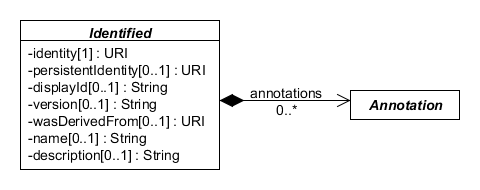
\includegraphics[scale=0.6]{uml/identified}
\caption[]{Diagram of the \sbol{Identified} abstract class and its associated properties}
\label{uml:identified}
\end{center}
\end{figure}

\subsubsection*{The \sbolheading{identity} property}
\label{sec:identity}
The \sbol{identity} property is REQUIRED by all \sbol{Identified} objects and has a data type of \external{URI}. A given \sbol{Identified} object's \sbol{identity} \external{URI} MUST be globally unique among all other \sbol{identity} \external{URI}s. It is also highly RECOMMENDED that the URI structure follows the recommended best-practices for compliant URIs specified in \ref{sec:compliant}.

Although most SBOL properties are defined by SBOL and serialized with its namespace, the \sbol{identity} property is defined by the analogous RDF \external{about} property and is serialized with the RDF namespace as follows:

\external{http://www.w3.org/1999/02/22-rdf-syntax-ns\#about}.

This substitution is in keeping with the commitment of the SBOL community to the practical reuse of existing standards.

\subsubsection*{The \sbolheading{persistentIdentity} property}
\label{sec:persistentIdentity}
The \sbol{persistentIdentity} property is OPTIONAL and has a data type of \external{URI}. This \external{URI} serves to uniquely refer to a set of SBOL objects that are different versions of each other. 

An \sbol{Identified} object MUST be referred to using either its \sbol{identity} \external{URI} or its \sbol{persistentIdentity} \external{URI}.

\subsubsection*{The \sbolheading{displayId} property}
\label{sec:displayId}
The \sbol{displayId} property is an OPTIONAL identifier with a data type of \external{String}. This property is intended to be an intermediate between \sbol{name} and \sbol{identity} that is machine-readable, but more human-readable than the full \external{URI} of an \sbol{identity}. 

If the \sbol{displayId} property is used, then its \external{String} value SHOULD be locally unique (global uniqueness is not required) and MUST be composed of only alphanumeric or underscore characters and MUST NOT begin with a digit.

% compliant with the type \external{http://www.w3.org/TR/xmlschema-2/\#NCName}, except that it must not include the characters "-" and ".". 

\subsubsection*{The \sbolheading{version} property}
\label{sec:version}

The \sbol{version} property is OPTIONAL and has a data type of \external{String}. This property can be used to compare two SBOL objects with the same \sbol{persistentIdentity}.

If the \sbol{version} property is used, then it is RECOMMENDED that version numbering should follow the conventions of semantic versioning (\url{http://semver.org/}), particularly as implemented by Maven (\url{http://maven.apache.org/}).
This convention represents versions as sequences of numbers and qualifiers that are separated by the characters ``{\tt .}'' and ``{\tt -}'' and are compared in lexicographical order (for example, 1 < 1.3.1 < 2.0-beta).
For a full explanation, see the linked resources.

\subsubsection*{The \sbolheading{wasDerivedFrom} property}
\label{sec:wasDerivedFrom}

The \sbol{wasDerivedFrom} property is OPTIONAL and has a data type of \external{URI}. An SBOL object with this property refers to another SBOL object or non-SBOL resource from which this object was derived. 

If the \sbol{wasDerivedFrom} property of an SBOL object $A$ refers to another SBOL object $B$ with the same \sbol{persistentIdentity}, and both $A$ and $B$ have a \sbol{version}, then the \sbol{version} of $B$ MUST come before that of $A$. In addition, an SBOL object MUST NOT refer to itself via its own \sbol{wasDerivedFrom} property or form a circular chain of references via its \sbol{wasDerivedFrom} property and those of other SBOL objects. For example, the reference chain ``$A$ was derived from $B$ and $B$ was derived from $A$'' is circular.

\subsubsection*{The \sbolheading{name} property}
\label{sec:name}

The \sbol{name} property is OPTIONAL and has a data type of \external{String}. This property is intended to be displayed to a human when visualizing an \sbol{Identified} object.

If an \sbol{Identified} object lacks a name, then software tools SHOULD instead display the object's \sbol{displayId} or \sbol{identity}.
It is RECOMMENDED that software tools give users the ability to switch perspectives between \sbol{name} properties that are human-readable and \sbol{displayId} properties that are less human-readable, but are more likely to be unique.

\subsubsection*{The \sbolheading{description} property}
\label{sec:description}

The \sbol{description} property is OPTIONAL and has a data type of \external{String}. This property is intended to contain a more thorough text description of an \sbol{Identified} object.

\subsubsection*{Serialization}

No complete serialization is defined for \sbol{Identified}, since this
class is only used indirectly through its child classes.  Any such
child class, however, has the following form for serializing
properties inherited from \sbol{Identified}, where CLASS\_NAME is
replaced by the name of the class:

\lstsetsbol
\begin{lstlisting}
<?xml version="1.0" ?>
<rdf:RDF xmlns:pr="http://partsregistry.org" xmlns:rdf="http://www.w3.org/1999/02/22-rdf-syntax-ns#" xmlns:dcterms="http://purl.org/dc/terms/" xmlns:prov="http://www.w3.org/ns/prov#" xmlns:sbol="http://sbols.org/v2#">
  <sbol:CLASS_NAME rdf:about="...">
    [\emph{zero or one}] <sbol:persistentIdentity rdf:resource="..."/> [\emph{element}]
    [\emph{zero or one}] <sbol:displayId>...</sbol:displayId> [\emph{element}]
    [\emph{zero or one}] <sbol:version>...</sbol:version> [\emph{element}]
    [\emph{zero or one}] <prov:wasDerivedFrom rdf:resource="..."/> [\emph{element}]
    [\emph{zero or one}] <dcterms:title>...</dcterms:title> [\emph{element}]
    [\emph{zero or one}] <dcterms:description>...</dcterms:description> [\emph{element}]
               ...
  </sbol:CLASS_NAME>
  ...
</rdf:RDF>
\end{lstlisting}

Note that several of the properties are not in the \external{sbol}
namespace, but are mapped to standardized terms defined elsewhere:
\begin{itemize}
\item \sbol{identity} is serialized as \external{rdf:about}
\item \sbol{wasDerivedFrom} is serialized as \external{prov:wasDerivedFrom}
\item \sbol{name} is serialized as \external{dcterms:title}
\item \sbol{description} is serialized as \external{dcterms:description}
\end{itemize}

% \subsection{Documented}
% \label{sec:Documented}
% The \sbol{Documented} abstract class is inherited by the classes of SBOL objects that can contain human-readable properties, such as name and description. This class extends \sbol{Identified} with two additional data properties: \sbol{name}, and \sbol{description} (\ref{uml:documented}). 

% \begin{figure}[ht]
% \begin{center}
% 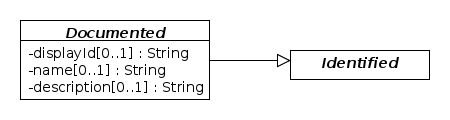
\includegraphics[scale=0.6]{uml/documented}
% \caption[]{The \sbol{Documented} abstract class.}
% \label{uml:documented}
% \end{center}
% \end{figure}

% \subsubsection*{Serialization}

% No complete serialization is defined for \sbol{Documented}, since this
% class is only used indirectly through its child classes.  Any such
% child class, however, has the following form for serializing
% properties inherited from \sbol{Documented}, where CLASS\_NAME is
% replaced by the name of the class:

\subsection {TopLevel}
\label{sec:TopLevel}
\sbol{TopLevel} is an abstract class that is extended by any \sbol{Identified} class that can be found at the top level of an SBOL document or file. In other words, \sbol{TopLevel} objects are not nested inside any other object via a composite aggregation or black diamond arrow association property. Instead of nesting, composite \sbol{TopLevel} objects refer to subordinate \sbol{TopLevel} objects by their URIs using shared aggregation or white diamond arrow association properties. The \sbol{TopLevel} classes defined in this specification are \sbol{Sequence}, \sbol{ComponentDefinition}, \sbol{Model}, \sbol{ModuleDefinition},  \sbol{Collection}, and \sbol{GenericTopLevel} (\ref{uml:toplevel}).

\begin{figure}[ht]
\begin{center}
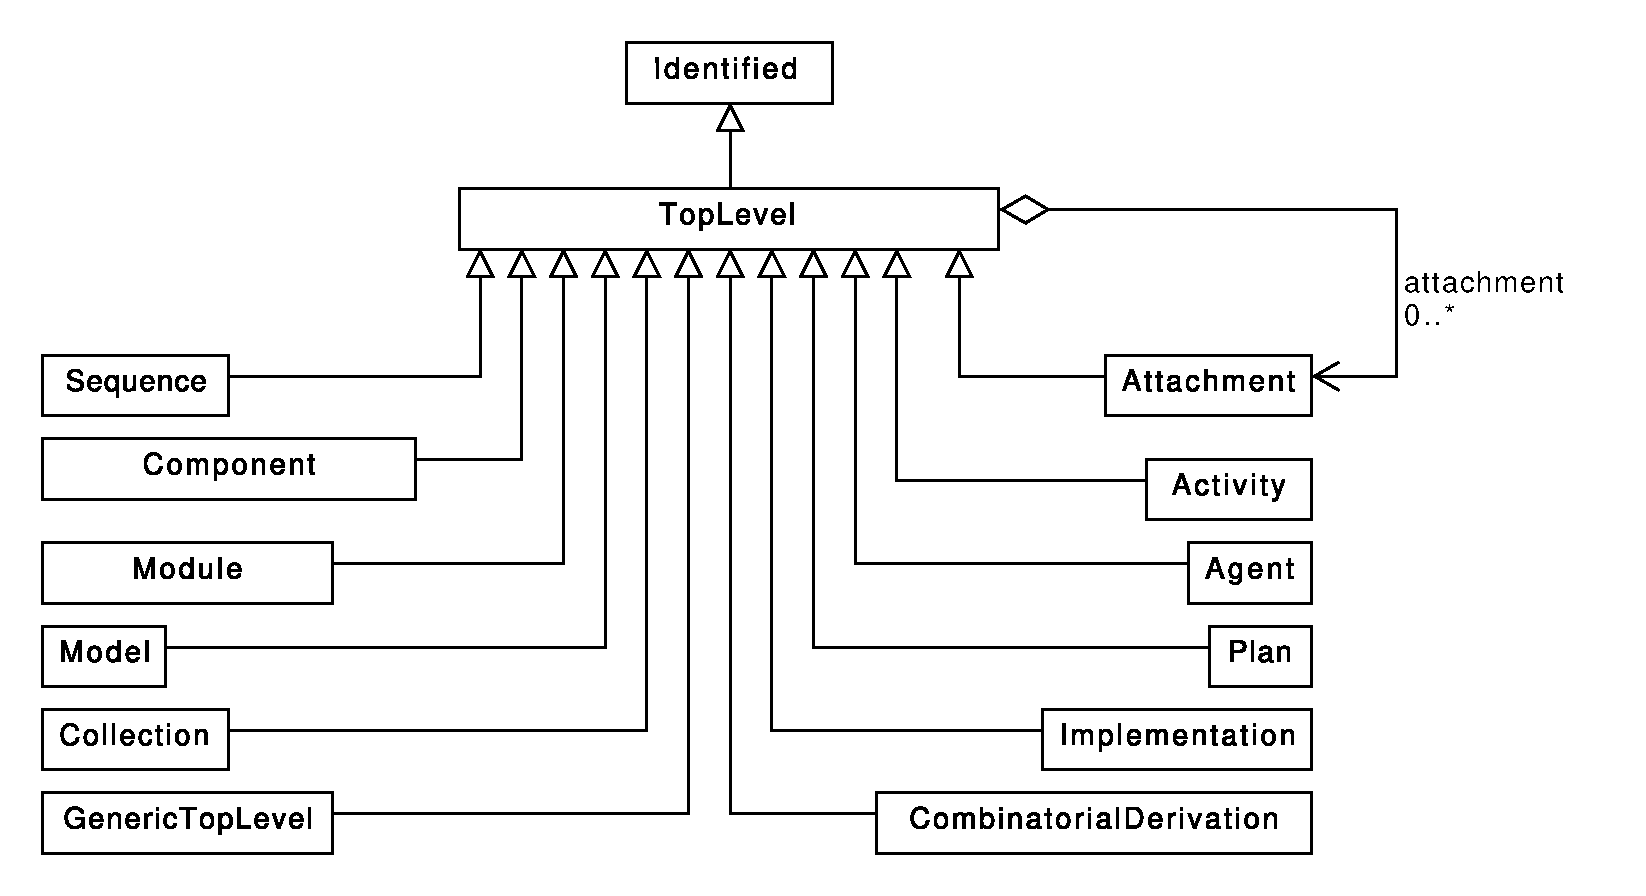
\includegraphics[width=\textwidth]{uml/toplevel}
\caption[]{Classes that inherit from the \sbol{TopLevel} abstract class.}
\label{uml:toplevel}
\end{center}
\end{figure}

\subsubsection*{Serialization}

No serialization is defined for \sbol{TopLevel}, since this class has
no properties of its own and is only used indirectly through its child
classes.

\subsection{Sequence}
\label{sec:Sequence}
The purpose of the \sbol{Sequence} class is to represent the primary structure of a \sbol{ComponentDefinition} object and the manner in which it is encoded. This representation is accomplished  by means of the \sbol{elements} property and \sbol{encoding} property (\ref{uml:sequence}).

\begin{figure}[ht]
\begin{center}
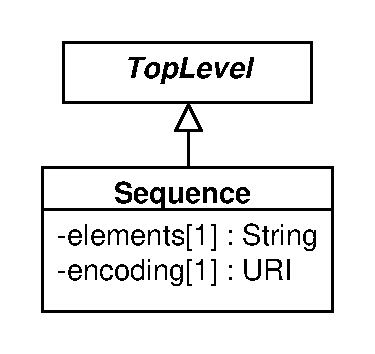
\includegraphics[scale=0.6]{uml/sequence}
\caption[]{Diagram of the \sbol{Sequence} class and its associated properties.}
\label{uml:sequence}
\end{center}
\end{figure}


\subsubsection*{The \sbolheading{elements} property}
\label{sec:elements}
The \sbol{elements} property is a REQUIRED \external{String} of characters that represents the constituents of a biological or chemical molecule. For example, these characters could represent the nucleotide bases of a molecule of DNA, the amino acid residues of a protein, or the atoms and chemical bonds of a small molecule.

\subsubsection*{The \sbolheading{encoding} property}
\label{sec:encoding}
The \sbol{encoding} property is REQUIRED and has a data type of \external{URI}. This property is used to indicate how the \sbol{elements} property of a \sbol{Sequence} MUST be formed and interpreted. 

For example, the \sbol{elements} property of a \sbol{Sequence} with an \external{IUPAC DNA} encoding property MUST contain characters that represent nucleotide bases, such as {\tt a}, {\tt t}, {\tt c}, and {\tt g}. The \sbol{elements} property of a \sbol{Sequence} with a \external{Simplified Molecular-Input Line-Entry System (SMILES)} encoding, on the other hand, MUST contain characters that represent atoms and chemical bonds, such as {\tt C}, {\tt N}, {\tt O}, and {\tt =}.

\ref{tbl:sequence_encodings} provides a list of RECOMMENDED \external{URI}s for the \sbol{encoding} property. The terms in \ref{tbl:sequence_encodings} are organized by the type of \sbol{ComponentDefinition} (see \ref{tbl:componentdefinition_types}) that typically refer to a \sbol{Sequence} with such an \sbol{encoding}. When the \sbol{encoding} of a \sbol{Sequence} is well described by one of the \external{URI}s in \ref{tbl:sequence_encodings}, it MUST use that \external{URI} for this property.

%A Summary of letters for nucleic acids and aminoacids
\begin{table}[ht]
  \begin{edtable}{tabular}{lll}
    \toprule
     \textbf{Encoding} & \textbf{URI} & \textbf{ComponentDefinition Type} \\
    \midrule
     IUPAC DNA, RNA & \url{http://www.chem.qmul.ac.uk/iubmb/misc/naseq.html} & DNA, RNA \\
    IUPAC Protein & \url{http://www.chem.qmul.ac.uk/iupac/AminoAcid/} & Protein\\
   SMILES & \url{http://www.opensmiles.org/opensmiles.html} & SmallMolecule \\
    \bottomrule
  \end{edtable}
  \caption{RECOMMENDED \external{URI}s for specifying the \sbol{encoding} property of a \sbol{Sequence}, organized by the type of \sbol{ComponentDefinition} (see \ref{tbl:componentdefinition_types}) that typically refer to a \sbol{Sequence} with such an \sbol{encoding}.}
  \label{tbl:sequence_encodings}
\end{table}

\subsubsection*{Serialization}
The serialization of a \sbol{Sequence} MUST have the following form:
\lstsetsbol
\begin{lstlisting}
<sbol:Sequence rdf:about="...">
      ...
  [\emph{one}] <sbol:elements>...</sbol:elements> [\emph{element}]
  [\emph{one}] <sbol:encoding rdf:resource="..."/> [\emph{element}]
</sbol:Sequence>
\end{lstlisting}

The example below shows the serialization of the \sbol{Sequence} for a promoter. The nucleotide bases of the \sbol{Sequence} are serialized as the \external{String} value of its \sbol{elements} property, while its \external{IUPAC DNA} encoding is serialized as the \external{URI} value of its  \sbol{encoding} property. 

\lstsetsbol
\begin{lstlisting}
<?xml version="1.0" ?>
<rdf:RDF xmlns:rdf="http://www.w3.org/1999/02/22-rdf-syntax-ns#" xmlns:dcterms="http://purl.org/dc/terms/" xmlns:prov="http://www.w3.org/ns/prov#" xmlns:sbol="http://sbols.org/v2#">
  <sbol:Sequence rdf:about="http://partsregistry.org/seq/BBa_J23119">
    <sbol:persistentIdentity rdf:resource="http://partsregistry.org/seq/BBa_J23119"/>
    <sbol:displayId>BBa_J23119</sbol:displayId>
    <prov:wasDerivedFrom rdf:resource="http://parts.igem.org/Part:BBa_J23119:Design"/>
    <sbol:elements>ttgacagctagctcagtcctaggtataatgctagc</sbol:elements>
    <sbol:encoding rdf:resource="http://www.chem.qmul.ac.uk/iubmb/misc/naseq.html"/>
  </sbol:Sequence>
</rdf:RDF>
\end{lstlisting}


\subsection{ComponentDefinition}
\label{sec:ComponentDefinition}

The \sbol{ComponentDefinition} class represents the structural entities of a biological design. The primary usage of this class is to represent structural entities with designed sequences, such as DNA, RNA, and proteins, but it can also be used to represent any other entity that is part of a design, such as small molecules, molecular complexes, and light. 

As shown in \ref{uml:component_definition}, the \sbol{ComponentDefinition} class describes a structural design entity using the following properties: \sbol{types}, \sbol{roles}, and \sbol{sequences}. In addition, this class has properties for describing and organizing the substructure of said design entity, including \sbol{components}, \sbol{sequenceConstraints}, and  \sbol{sequenceAnnotations}.

\begin{figure}[ht]
\begin{center}
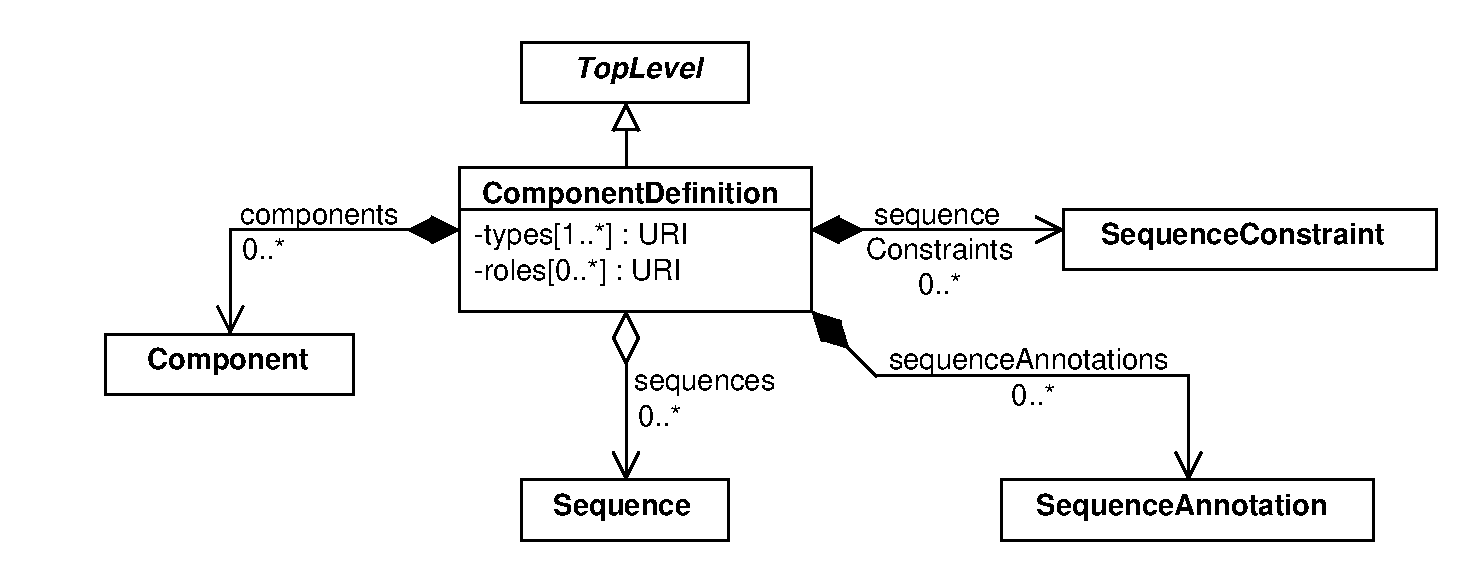
\includegraphics[width=0.95\textwidth]{uml/component_definition}
\caption[]{Diagram of the \sbol{ComponentDefinition} class and its associated properties.}
\label{uml:component_definition}
\end{center}
\end{figure}

\subsubsection*{The \sbolheading{types} property}
\label{sec:types}

The \sbol{types} property is a REQUIRED set of \external{URI}s that specifies the category of biochemical or physical entity (for example DNA, protein, or small molecule) that a \sbol{ComponentDefinition} object abstracts for the purpose of engineering design. 

The \sbol{types} property of every \sbol{ComponentDefinition} MUST contain one or more \external{URI}s that MUST identify terms from appropriate ontologies, such as the BioPAX ontology or the ontology of Chemical Entities of Biological Interest (ChEBI). \ref{tbl:componentdefinition_types} provides a list of RECOMMENDED ontology terms for the \sbol{types} property and their \external{URI}s. In order to maximize the compatibility of designs, any \sbol{ComponentDefinition} that can be well-described by one of the terms in \ref{tbl:componentdefinition_types} MUST use that term as one of its \sbol{types}. Finally, if the \sbol{types} property contains multiple \external{URIs}, then they MUST identify synonymous terms. 

\begin{table}[ht]
  \begin{edtable}{tabular}{ll}
    \toprule
    \textbf{ComponentDefinition Type} & \textbf{URI for BioPAX Term} \\
    \midrule
    DNA  & \url{http://www.biopax.org/release/biopax-level3.owl#DnaRegion}\\
    RNA  & \url{http://www.biopax.org/release/biopax-level3.owl#RnaRegion}\\
    Protein  & \url{http://www.biopax.org/release/biopax-level3.owl#Protein}\\
    Small Molecule  & \url{http://www.biopax.org/release/biopax-level3.owl#SmallMolecule}\\  
    \bottomrule
  \end{edtable}
  \caption{RECOMMENDED BioPAX terms to specify the \sbol{types} property of a \sbol{ComponentDefinition}.}
 \label{tbl:componentdefinition_types}
\end{table}

\subsubsection*{The \sbolheading{roles} property}
\label{sec:roles}

The \sbol{roles} property is an OPTIONAL set of \external{URI}s that clarifies the potential function of a \sbol{ComponentDefinition} in a biological context.

The \sbol{roles} property of a \sbol{ComponentDefinition} MAY contain one or more \external{URI}s that MUST identify terms from ontologies that are consistent with the \sbol{types} property of the \sbol{ComponentDefinition}. For example, the \sbol{roles} property of a DNA or RNA \sbol{ComponentDefinition} could contain \external{URI}s identifying terms from the Sequence Ontology (SO). \ref{tbl:componentdefinition_roles} contains a list of RECOMMENDED ontology terms for the \sbol{roles} property and their \external{URI}s. These terms are organized by the type of \sbol{ComponentDefinition} to which they SHOULD apply (see \ref{tbl:componentdefinition_types}). Any \sbol{ComponentDefinition} that can be well-described by one of the terms in \ref{tbl:componentdefinition_roles} MUST use that term as one of its \sbol{roles}. 

\begin{table}[ht]
  \begin{edtable}{tabular}{lll}
    \toprule
    \textbf{ComponentDefinition Role} & \textbf{URI for Ontology Term} & \textbf{ComponentDefinition Type} \\
    \midrule
   Promoter & \url{http://identifiers.org/so/SO:0000167} & DNA \\
   RBS & \url{http://identifiers.org/so/SO:0000139} & DNA \\
      CDS & \url{http://identifiers.org/so/SO:0000316} & DNA \\
      Terminator & \url{http://identifiers.org/so/SO:0000141} & DNA \\ 
      Gene & \url{http://identifiers.org/so/SO:0000704} & DNA \\
      mRNA & \url{http://identifiers.org/so/SO:0000234} & RNA \\ 
      Effector & \url{http://identifiers.org/chebi/CHEBI:35224} & Small Molecule \\
    \bottomrule
  \end{edtable}
  \caption{RECOMMENDED ontology terms to specify the \sbol{roles} property of a \sbol{ComponentDefinition}, organized by the type of \sbol{ComponentDefinition} to which they should apply (see \ref{tbl:componentdefinition_types}).}
  \label{tbl:componentdefinition_roles}
\end{table}

\NVtodo{Goksel to replace URI for Transcription Factor role with something more appropriate (currently is URI for the term ``transcription activity.''}

\subsubsection*{The \sbolheading{components} property}
\label{sec:components}

The \sbol{components} property is OPTIONAL and MAY specify a set of \sbol{Component} objects contained by its \sbol{ComponentDefinition}.

While the \sbol{ComponentDefinition} class is analogous to a blueprint or specification sheet for a biological part, the \sbol{Component} class represents the specific occurrence of a part within a design. Hence, this class allows a biological design to include multiple copies of a particular part. For example, the \sbol{ComponentDefinition} of a polycistronic gene could contain two \sbol{Component} objects that refer to the same \sbol{ComponentDefinition} of a CDS.

If the \sbol{ComponentDefinition} refers to one or more \sbol{Sequence} objects, then at least one of them MUST have the same \sbol{encoding} as a \sbol{Sequence} from the \sbol{ComponentDefinition} of each \sbol{Component} in the \sbol{components} property. In addition, it MUST be possible to align the \sbol{elements} of the latter \sbol{encoding}-matched \sbol{Sequence} objects to the former. For example, a DNA \sbol{ComponentDefinition} could have a \sbol{Sequence} with an \external{IUPAC DNA} \sbol{encoding} and \sbol{elements} ``{\tt gattaca}.'' In this case, any \sbol{Component} contained by this \sbol{ComponentDefinition} would itself need to have a \sbol{ComponentDefinition} that refers to a \sbol{Sequence} with an \external{IUPAC DNA} \sbol{encoding} and \sbol{elements} that can be aligned with ``{\tt gattaca},'' such as ``{\tt gatta}'' or ``{\tt ttaca}.''

% Furthermore, this \sbol{Sequence} MUST have the same \external{IUPAC} \sbol{encoding} as a \sbol{Sequence} of the parent \sbol{ComponentDefinition} that contains the \sbol{SequenceAnnotation}. 

\subsubsection*{The \sbolheading{sequences} property}
\label{sec:sequences}
The \sbol{sequences} property is OPTIONAL and MAY include a set of \external{URI}s that refer to \sbol{Sequence} objects. These objects define the primary structure of the \sbol{ComponentDefinition}.

Many \sbol{ComponentDefinition} objects will refer to precisely one \sbol{Sequence} object. For certain use cases, however, it may be appropriate to refer to multiple \sbol{Sequence} objects. For example, a user may wish to provide two different representations of the structure of a DNA \sbol{ComponentDefinition}, one that captures its primary structure at the level of nucleotide bases and one that captures its secondary and tertiary structure at the level of atoms and bonds. 

If a \sbol{ComponentDefinition} refers to more than one \sbol{Sequence} object, then these objects MUST be consistent with each other, such that well-defined mappings exist between their \sbol{elements} properties in accordance with their \sbol{encoding} properties. In addition, a \sbol{ComponentDefinition} MUST NOT refer to more than one \sbol{Sequence} with an \external{IUPAC} \sbol{encoding} (see \ref{tbl:sequence_encodings}). 

Finally, if a \sbol{ComponentDefinition} refers to one or more \sbol{Sequence} objects and its \sbol{types} property refers to a term from \ref{tbl:componentdefinition_types}, then at least one of these \sbol{Sequence} objects MUST have the \sbol{encoding} from \ref{tbl:sequence_encodings} that corresponds to this term.  Conversely, if a \sbol{ComponentDefinition} refers to a \sbol{Sequence} with an \sbol{encoding} from \ref{tbl:sequence_encodings}, then its \sbol{types} property MUST refer to the corresponding term from \ref{tbl:componentdefinition_types}. For example, if the \sbol{types} property of a \sbol{ComponentDefinition} refers to the BioPAX term for DNA, then one of the \sbol{Sequence} objects to which it refers (if any) MUST have an \external{IUPAC DNA} \sbol{encoding}, and if a \sbol{ComponentDefinition} refers to a \sbol{Sequence} with an an \external{IUPAC DNA} \sbol{encoding}, then its \sbol{types} property must refer to the BioPAX term for DNA.

\subsubsection*{The \sbolheading{sequenceConstraints} property}
\label{sec:sequenceConstraints}

The \sbol{sequenceConstraints} property is OPTIONAL and MAY contain a set of \sbol{SequenceConstraint} objects. These objects describe any restrictions on the relative, sequence-based positions of the \sbol{Component} objects contained by the \sbol{ComponentDefinition}. For example, the \sbol{ComponentDefinition} of a gene may specify that its promoter \sbol{Component} precedes its CDS \sbol{Component}. This is particulary useful when a \sbol{ComponentDefinition} lacks a \sbol{Sequence} and therefore cannot specify the precise, sequence-based positions of its \sbol{Component} objects using \sbol{SequenceAnnotation} objects.

\subsubsection*{The \sbolheading{sequenceAnnotations} property}
\label{sec:sequenceAnnotations}

The \sbol{sequenceAnnotations} property is OPTIONAL and MAY contain a set of \sbol{SequenceAnnotation} objects. Each \sbol{SequenceAnnotation} specifies and describes a potentially discontiguous region on the \sbol{Sequence} objects referred to by the \sbol{ComponentDefinition}. In addition, each \sbol{SequenceAnnotation} can  position a \sbol{Component} of the \sbol{ComponentDefinition} at the region specified by its \sbol{Location} objects (see \ref{sec:Location}).

If the \sbol{ComponentDefinition} does not refer to a \sbol{Sequence} with an \external{IUPAC} \sbol{encoding} from \ref{tbl:sequence_encodings}, then it MUST NOT contain any \sbol{SequenceAnnotation} with a \sbol{Range} or \sbol{Cut} \sbol{Location}. By contrast, if the \sbol{ComponentDefinition} does refer to a \sbol{Sequence} with an \sbol{IUPAC} \sbol{encoding}, then each \sbol{SequenceAnnotation} it contains with a \sbol{Range} and/or \sbol{Cut} MUST cover a region on the \sbol{elements} of this \sbol{Sequence}. For example, the \sbol{ComponentDefinition} of a eukaryotic gene could refer to a \sbol{Sequence} with an \external{IUPAC DNA} \sbol{encoding}. In order to specify the discontiguous region occupied by its CDS, this gene \sbol{ComponentDefinition} would need a \sbol{SequenceAnnotation} that contains one or more \sbol{Range} objects, each one specifying \sbol{start} and \sbol{end} positions that are consistent with the \sbol{elements} of its DNA \sbol{Sequence}.

\subsubsection*{Serialization}
The serialization of a \sbol{ComponentDefinition} MUST have the form below. The \sbol{sequences}, \sbol{components},  \sbol{sequenceConstraints}, and \sbol{sequenceAnnotations} properties of a \sbol{ComponentDefinition} contain objects belonging to the appropriate SBOL classes as their values, while the \sbol{types} and \sbol{roles} properties contain \external{URI}s that identify ontology terms as their values. As shown below, each one of these objects and \external{URI}s is serialized as part of an implicit set of SBOL properties with singular rather then plural names. In particular, each object is serialized as a RDF/XML node nested within a singular property, while each \external{URI} is serialized as a \external{rdf:resource} on a singular property.

\lstsetsbol
\begin{lstlisting}
<sbol:ComponentDefinition rdf:about="...">
               ...
  [\emph{zero or more}]  <sbol:sequence rdf:resource="..."/> [\emph{element}]
  [\emph{one or more}]   <sbol:type rdf:resource="..."/> [\emph{elements}]
  [\emph{zero or more}]  <sbol:role rdf:resource="..."/> [\emph{elements}]    
  [\emph{zero or more}]  <sbol:component>
                 <sbol:Component rdf:about="...">...</sbol:Component>
               </sbol:component> [\emph{elements}]
  [\emph{zero or more}] <sbol:sequenceAnnotation>
                 <sbol:SequenceAnnotation rdf:about="...">...</sbol:SequenceAnnotation>
               </sbol:sequenceAnnotation> [\emph{elements}]        
  [\emph{zero or more}] <sbol:sequenceConstraint>
                 <sbol:SequenceConstraint rdf:about="...">...</sbol:SequenceConstraint>
               </sbol:sequenceConstraint> [\emph{elements}]        
</sbol:ComponentDefinition>
\end{lstlisting}


The example below shows the serialization for the \sbol{ComponentDefinition} of a promoter. The BioPAX term \external{DnaRegion} and the ChEBI term \external{CHEBI:4705} (\external{double-stranded DNA}) are used to indicate that the type of biological entity represented by this \sbol{ComponentDefinition} is DNA. Its role is specified using the SO terms \external{SO:0000167} (\external{promoter}) and the more specific \external{SO:0000613} (\external{bacterial\_RNApol\_promoter}).

\lstsetsbol
\begin{lstlisting}
<?xml version="1.0" ?>
<rdf:RDF xmlns:rdf="http://www.w3.org/1999/02/22-rdf-syntax-ns#" xmlns:dcterms="http://purl.org/dc/terms/" xmlns:prov="http://www.w3.org/ns/prov#" xmlns:sbol="http://sbols.org/v2#">
  <sbol:ComponentDefinition rdf:about="http://partsregistry.org/cd/BBa_J23119">
    <sbol:persistentIdentity rdf:resource="http://partsregistry.org/cd/BBa_J23119"/>
    <sbol:displayId>BBa_J23119</sbol:displayId>
    <prov:wasDerivedFrom rdf:resource="http://partsregistry.org/Part:BBa_J23119"/>
    <dcterms:title>J23119 promoter</dcterms:title>
    <dcterms:description>Constitutive promoter</dcterms:description>
    <sbol:type rdf:resource="http://identifiers.org/chebi/CHEBI:4705"/>
    <sbol:type rdf:resource="http://www.biopax.org/release/biopax-level3.owl#DnaRegion"/>
    <sbol:role rdf:resource="http://identifiers.org/so/SO:0000167"/>
    <sbol:role rdf:resource="http://identifiers.org/so/SO:0000613"/>
    <sbol:sequence rdf:resource="http://partsregistry.org/seq/BBa_J23119"/>
  </sbol:ComponentDefinition>
</rdf:RDF>
\end{lstlisting}


\subsubsection{ComponentInstance}
\label{sec:ComponentInstance}

\begin{figure}[ht]
\begin{center}
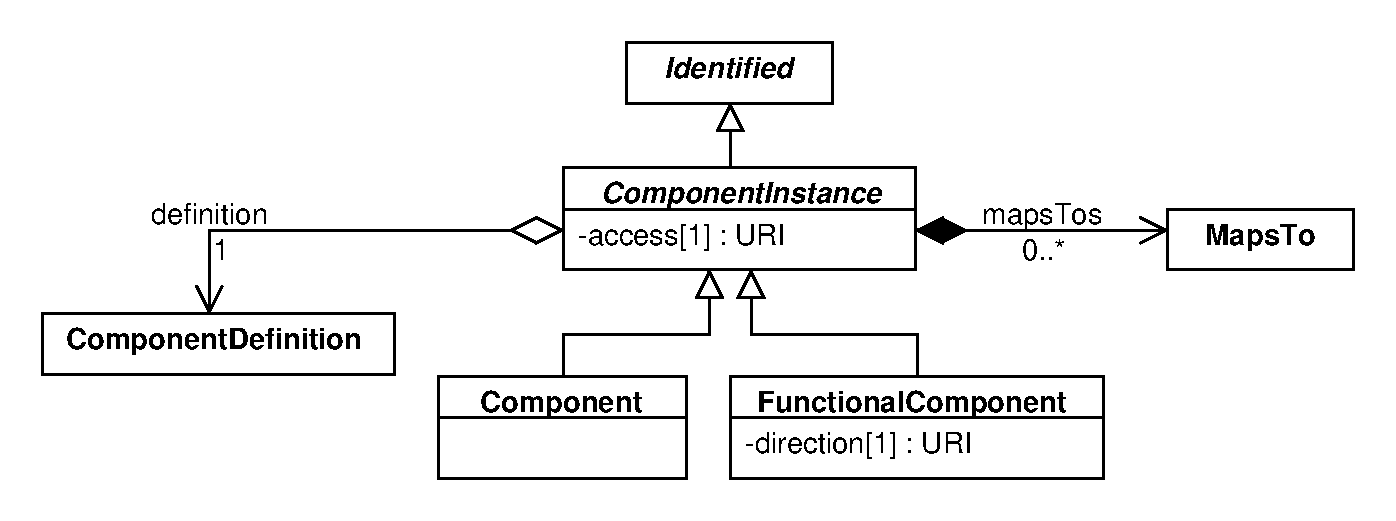
\includegraphics[scale=0.6]{uml/component_instance}
\caption[]{Diagram of the \sbol{ComponentInstance} class and its associated properties.}
\label{uml:component}
\end{center}
\end{figure}

The \sbol{ComponentInstance} abstract class is inherited by SBOL classes that represent the usage or occurrence of a \sbol{ComponentDefinition} within a larger design (that is, another \sbol{ComponentDefinition} or \sbol{ModuleDefinition}). Currently, there are two subclasses of \sbol{ComponentInstance}:
\begin{itemize}
\item The \sbol{Component} class is used to specify the structural usage of a \sbol{ComponentDefinition} inside another \sbol{ComponentDefinition} via the \sbol{components} property.
\item The \sbol{FunctionalComponent} class is used to specify the functional usage of a \sbol{ComponentDefinition} inside a \sbol{ModuleDefinition} via the \sbol{functionalComponents} property. This class is described in \ref{sec:FunctionalComponent}.
\end{itemize}

\paragraph{The \sbolheading{definition} property}
\label{sec:definition}

The \sbol{definition} property is a REQUIRED \external{URI} that refers to the \sbol{ComponentDefinition} of the \sbol{ComponentInstance}. As described in the previous section, this \sbol{ComponentDefinition} effectively provides information about the \sbol{types} and \sbol{roles} of the \sbol{ComponentInstance}.

The \sbol{definition} property MUST NOT refer to the same \sbol{ComponentDefinition} as that which contains the \sbol{ComponentInstance}. Furthermore, \sbol{ComponentInstance} objects MUST NOT form a circular chain of references via their \sbol{definition} properties and the \sbol{ComponentDefinition} objects that contain them. For example, consider the \sbol{ComponentInstance} objects $A$ and $B$ and the \sbol{ComponentDefinition} objects $X$ and $Y$. The reference chain ``$X$ contains $A$, $A$ is defined by $Y$, $Y$ contains $B$, and $B$ is defined by $X$'' is circular. 

\paragraph{The \sbolheading{mapsTos} property}\label{sec:mapsTos}

The \sbol{mapsTos} property is OPTIONAL and MAY contain a set of \sbol{MapsTo} objects that refer to and link together \sbol{ComponentInstance} objects (both \sbol{Component} objects and \sbol{FunctionalComponent} objects)  within a larger design.

\ref{sec:MapsTo} contains a more detailed description of the \sbol{MapsTo} class.

\paragraph{The \sbolheading{access} property}
\label{sec:access}

The \sbol{access} property is a REQUIRED \external{URI} that indicates whether the \sbol{ComponentInstance} 
can be referred to by a \sbol{MapsTo}.

\ref{tbl:componentInstance_access} provides a list of REQUIRED \sbol{access} \external{URI}s. The value of the \sbol{access} property MUST be one of these \external{URI}s.

\begin{table}[ht]
  \begin{edtable}{tabular}{lp{4in}}
    \toprule
    \textbf{URI} & \textbf{Access Description} \\
    \midrule
    \url{http://sbols.org/v2#public}  & The \sbol{ComponentInstance} MAY be referred to by \sbol{MapsTo} objects. \\
        \url{http://sbols.org/v2#private}  & The \sbol{ComponentInstance} MUST NOT be referred to by any \sbol{MapsTo} object. \\
    \bottomrule
  \end{edtable}
  \caption{REQUIRED \external{URI}s for the \sbol{access} property.}
  \label{tbl:componentInstance_access}
\end{table}

Unless a designer has a reason to prevent others from accessing the \sbol{ComponentInstance} when their design is reused, it is RECOMMENDED that the \sbol{access} property of the \sbol{ComponentInstance} be set to ``public.''
For example, a designer who is concerned about retroactivity may set the \sbol{access} of the \sbol{ComponentInstance} to ``private'' in order to prevent others from specifying its \sbol{Participation} in a new \sbol{Interaction} as part of a composite design.

\paragraph{Serialization}

No serialization is defined for the \sbol{ComponentInstance} class, since this class is only used indirectly through the \sbol{Component} and \sbol{FunctionalComponent} subclasses.

\subsubsection{Component}
\label{sec:Component}
The \sbol{Component} class is used to compose \sbol{ComponentDefinition} objects into a structural hierarchy. For example, the \sbol{ComponentDefinition} of a gene could contain four \sbol{Component} objects, including a promoter, RBS, CDS, and terminator. In turn, the \sbol{ComponentDefinition} of the promoter \sbol{Component} could contain \sbol{Component} objects defined as various operator sites.

% All \sbol{Component} objects directly referenced within a \sbol{ComponentDefinition}'s \sbol{SequenceAnnotation} or \sbol{SequenceConstraint} parts MUST be associated with that \sbol{ComponentDefinition} by means of its \sbol{components} property.

\paragraph{Serialization}

The serialization of a \sbol{Component} MUST have the following form:

\lstsetsbol
\begin{lstlisting}
<sbol:Component rdf:about="...">
               ...
  [\emph{one}]          <sbol:access rdf:resource="..."/> [\emph{element}]
  [\emph{one}]          <sbol:definition rdf:resource="..."/> [\emph{element}]    
  [\emph{zero or more}] <sbol:mapsTo rdf:resource="..."/> [\emph{elements}]
</sbol:Component>
\end{lstlisting}

The example below shows the serialization of a \sbol{Component}
that represents an instance of a promoter:

\lstsetsbol
\begin{lstlisting}
<sbol:Component rdf:about="http://partsregistry.org/cd/BBa_F2620/pLuxR">
  <sbol:persistentIdentity rdf:resource="http://partsregistry.org/cd/BBa_F2620/pLuxR"/>
  <sbol:displayId>pLuxR</sbol:displayId>
  <sbol:access rdf:resource="http://sbols.org/v2#public"/>
  <sbol:definition rdf:resource="http://partsregistry.org/cd/BBa_R0062"/>
</sbol:Component>
\end{lstlisting}



\subsubsection{MapsTo}
\label{sec:MapsTo}

\begin{figure}[ht]
\begin{center}
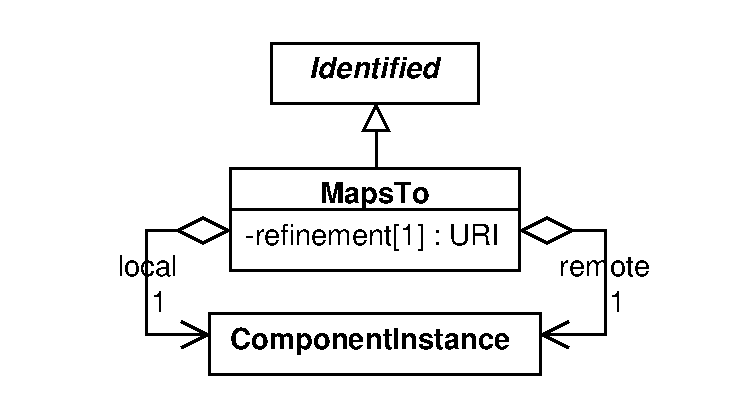
\includegraphics[scale=0.6]{uml/maps_to}
\caption[]{Diagram of the \sbol{MapsTo} class and its associated properties.}
\label{uml:maps_to}
\end{center}
\end{figure}

When \sbol{ComponentDefinition} and \sbol{ModuleDefinition} objects are composed into a structural and functional hierarchies using \sbol{ComponentInstance} and \sbol{Module} objects, it is often the case that some \sbol{ComponentInstance} objects are intended to represent the same entity in the overall design. The purpose of the \sbol{MapsTo} class is to make these identity relationships clear and explicit.

In particular, a \sbol{MapsTo} object provides two pieces of information:
\begin{itemize}
\item An identity relationship between two \sbol{ComponentInstance} objects, the first contained by the ``lower level'' definition of the \sbol{ComponentInstance} or \sbol{Module} that owns the
  \sbol{MapsTo}, and the second contained by the ``higher level'' definition that contains this \sbol{ComponentInstance} or \sbol{Module}. The \sbol{remote} property of a \sbol{MapsTo} refers to the first ``lower level'' \sbol{ComponentInstance}, while the \sbol{local} property refers to the second ``higher level'' \sbol{ComponentInstance}.
\item Instructions on what to do if the \sbol{local} and \sbol{remote} \sbol{ComponentInstance} objects refer to different \sbol{ComponentDefinition} objects (that is, they are not identical). These are specified using the \sbol{refinement} property of the \sbol{MapsTo} class.
\end{itemize}

\begin{figure}[ht]
\begin{center}
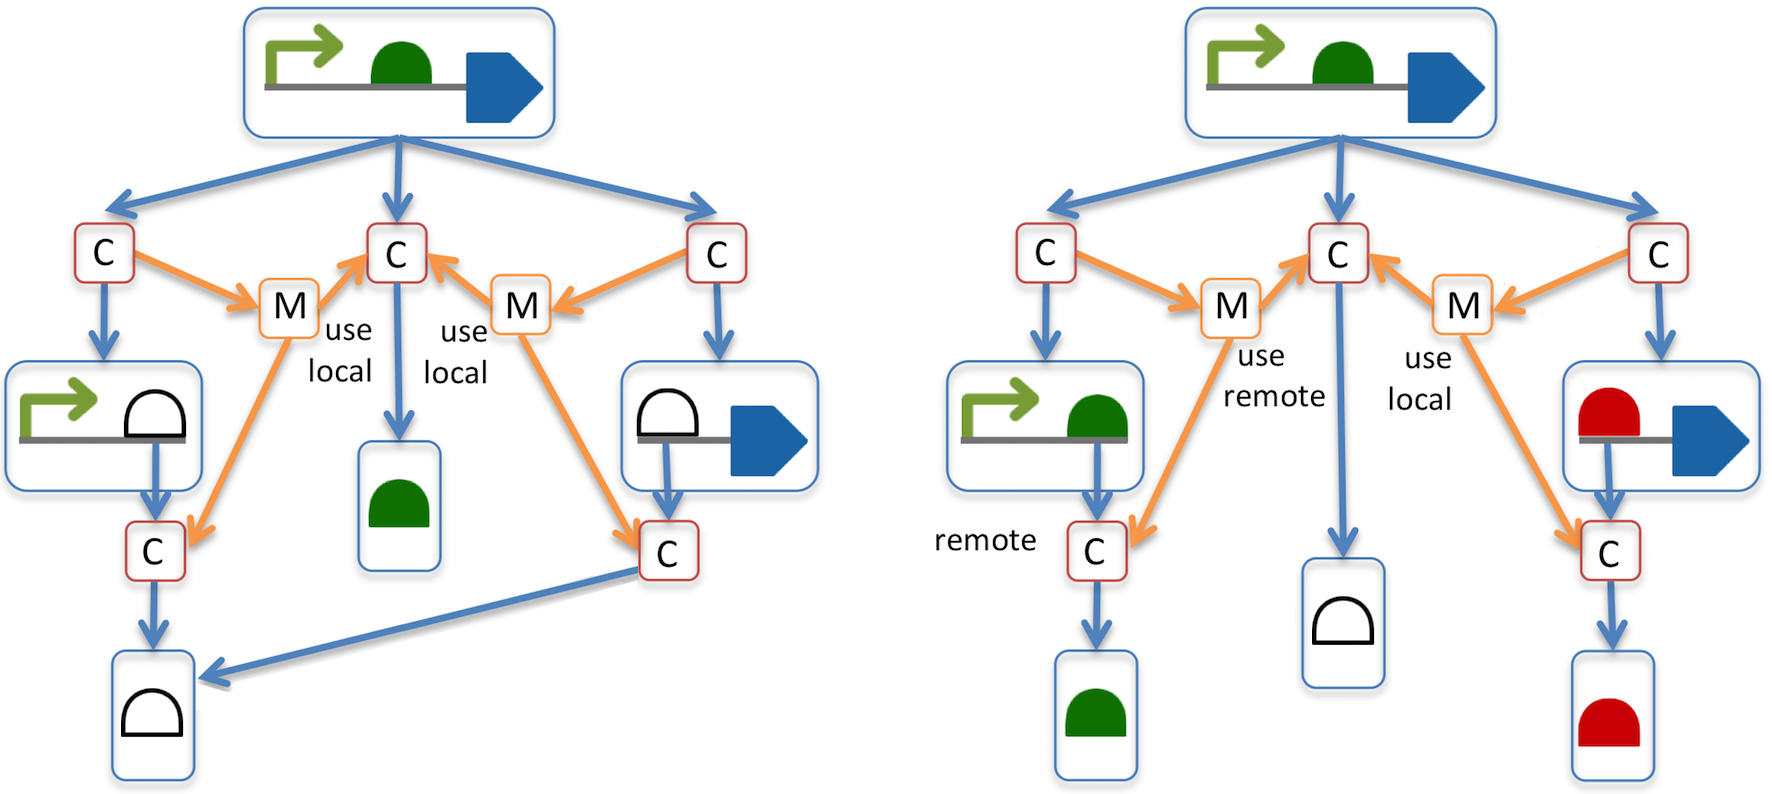
\includegraphics[scale=1]{images/MapsTo_Diagram3}
\caption{Linking \sbol{Component} objects using \sbol{MapsTo} entities. Boxes with diagrams represent \sbol{ComponentDefinition} objects, boxes with the C label represent \sbol{Component} objects, and boxes with the M label represent \sbol{MapsTo} objects. In both diagrams, a promoter-RBS \sbol{ComponentDefinition} and a RBS-CDS \sbol{ComponentDefinition} are being composed to form the \sbol{ComponentDefinition} of a complete transcriptional unit. In the lefthand diagram, the two \sbol{Component} objects inside the promoter-RBS \sbol{ComponentDefinition} and RBS-CDS \sbol{ComponentDefinition} objects both refer to an abstract RBS \sbol{ComponentDefinition} that lacks a sequence (white semicircle). Through the use of \sbol{MapsTo} objects with \sbol{refinement} set to useLocal, these ``lower level'' \sbol{ComponentDefinition} objects are effectively overridden by that of the green RBS in the \sbol{ComponentDefinition} of the complete transcriptional unit. In the righthand diagram, however, the two ``lower level'' RBS \sbol{ComponentDefinition} objects do not lack sequences and it is the ``higher level'' RBS \sbol{ComponentDefinition} that is abstract. In this case, one of the \sbol{MapsTo} objects has a useRemote \sbol{refinement}, resulting in the green RBS \sbol{ComponentDefinition} overriding that of the abstract RBS in the ``higher level'' \sbol{ComponentDefinition}.}
\label{image:maps_to_diagram2}
\end{center}
\end{figure}

To illustrate this concept, two examples are provided in \ref{image:maps_to_diagram2}, in which the \sbol{ComponentDefinition} of a transcriptional unit is specified by composing two ``lower level'' \sbol{ComponentDefinition} objects.
In both examples, the two ``lower level'' \sbol{ComponentDefinition} objects each contain a RBS \sbol{Component} that is intended to represent the same design entity in the ``higher level'' \sbol{ComponentDefinition} of the transcriptional unit.

In order to explicitly represent the identity relationships in this example, a new RBS \sbol{Component} needs to be created inside the ``higher level'' \sbol{ComponentDefinition}.
This ``higher level'' \sbol{Component} then needs to be linked to the equivalent ``lower level'' \sbol{Component} objects by means of the \sbol{MapsTo} class, using one \sbol{MapsTo} object per link.  
For example, in order to link the ``higher level'' RBS \sbol{Component} to the ``lower level'' RBS \sbol{Component} of the promoter-RBS \sbol{ComponentDefinition}, a \sbol{MapsTo} must be created on the ``higher level'' promoter-RBS \sbol{Component}. The \sbol{local} property of this \sbol{MapsTo} must then refer to the ``higher level'' RBS \sbol{Component}, while its \sbol{remote} property must refer to the ``lower level'' RBS \sbol{Component}.
In this way, many ``lower level'' \sbol{Component} objects can be linked together at the ``higher level'' using as an equal number of \sbol{MapsTo} objects, each one referring to a different \sbol{remote} \sbol{Component}, but all referring to the same \sbol{local} \sbol{Component}.

The same types of identity relationships can also be declared between \sbol{FunctionalComponent} objects contained by \sbol{ModuleDefinition} objects, or between \sbol{Component} objects and \sbol{FunctionalComponent} objects contained by \sbol{ComponentDefinition} objects and \sbol{ModuleDefinition} objects, respectively. See \ref{sec:examples} and \ref{ser:examples} for additional examples using the \sbol{MapsTo} class.

\paragraph{The \sbolheading{local} property}\label{sec:local}
This REQUIRED property has a data type of \external{URI} and is used to refer to the \sbol{ComponentInstance} contained by the ``higher level'' \sbol{ComponentDefinition} or \sbol{ModuleDefinition}. This \sbol{local} \sbol{ComponentInstance} MUST be contained by the \sbol{ComponentDefinition} or \sbol{ModuleDefinition} that contains the \sbol{ComponentInstance} or \sbol{Module} that owns the \sbol{MapsTo}. Finally, the \sbol{access} property of the \sbol{local} \sbol{ComponentInstance} MUST be set to ``public.''

\paragraph{The \sbolheading{remote} property}\label{sec:remote}
This REQUIRED property has a data type of \external{URI} and is used to refer to the \sbol{ComponentInstance} contained by the ``lower level'' \sbol{ComponentDefinition} or \sbol{ModuleDefinition}.  This \sbol{remote} \sbol{ComponentInstance} MUST be contained by the \sbol{ComponentDefinition} or \sbol{ModuleDefinition} that is the \sbol{definition} of the \sbol{ComponentInstance} or \sbol{Module} that owns the \sbol{MapsTo}. Lastly, the \sbol{access} property of the \sbol{remote} \sbol{ComponentInstance} MUST be set to ``public.''
 
\paragraph{The \sbolheading{refinement} property}\label{sec:refinement}
The \sbol{refinement} property is REQUIRED and has a data type of \external{URI}. Each \sbol{MapsTo} object MUST specify the relationship between its \sbol{local} and \sbol{remote} \sbol{ComponentInstance} objects using one of the REQUIRED \sbol{refinement} \external{URI}s provided in \ref{tbl:mapsto_refinement}.

\begin{table}[ht]
  \begin{edtable}{tabular}{lp{4in}}
    \toprule
    \textbf{Refinement URI} & \textbf{Description} \\
    \midrule
    \url{http://sbols.org/v2#useRemote}  & All references to the \sbol{definition} property of the \sbol{local}  \sbol{ComponentInstance} MUST dereference to that of the \sbol{remote} \sbol{ComponentInstance} instead.\\
    \url{http://sbols.org/v2#useLocal}  & In the context of the \sbol{ComponentDefinition} or \sbol{ModuleDefinition} that contains the owner of the \sbol{MapsTo}, all references to the \sbol{definition} property of the \sbol{remote}  \sbol{ComponentInstance} MUST dereference to that of the \sbol{local} \sbol{ComponentInstance} instead.\\
    \url{http://sbols.org/v2#verifyIdentical}  & The \sbol{definition} properties of the \sbol{local} and \sbol{remote} \sbol{ComponentInstance} objects MUST refer to the same \sbol{ComponentDefinition}.\\
        \url{http://sbols.org/v2#merge}  & In the context of the \sbol{ComponentDefinition} or \sbol{ModuleDefinition} that contains the owner of the \sbol{MapsTo}, all references to the \sbol{definition} property of the \sbol{local} \sbol{ComponentInstance} or that of the \sbol{remote} \sbol{ComponentInstance} MUST dereference to both such properties.\\
    \bottomrule
  \end{edtable}
  \caption{REQUIRED \external{URI}s for the \sbol{refinement} property.}
  \label{tbl:mapsto_refinement}
\end{table}

\paragraph{Serialization}
The serialization of \sbol{MapsTo} MUST have the following form.
\lstsetsbol
\begin{lstlisting}
<sbol:MapsTo rdf:about="...">
      ...
  [\emph{one}] <sbol:refinement rdf:resource="..."/> [\emph{element}]
  [\emph{one}] <sbol:remote rdf:resource="..."/> [\emph{element}]
  [\emph{one}] <sbol:local rdf:resource="..."/> [\emph{element}]
</sbol:MapsTo>
\end{lstlisting}

In the example below, a \sbol{FunctionalComponent} in a ``lower level'' LacI inverter \sbol{ModuleDefinition} is linked to a \sbol{FunctionalComponent} in a ``higher level'' \sbol{ModuleDefinition} of a genetic toggle switch. The full example can be found in \ref{ser:toggleswitch}.
\lstsetsbol
\begin{lstlisting}
<sbol:MapsTo rdf:about="http://sbolstandard.org/example/toggle_switch/laci_inverter/LacI_mapping">
  <sbol:persistentIdentity rdf:resource="http://sbolstandard.org/example/toggle_switch/laci_inverter/LacI_mapping"/>
  <sbol:displayId>LacI_mapping</sbol:displayId>
  <sbol:refinement rdf:resource="http://sbols.org/v2#useRemote"/>
  <sbol:remote rdf:resource="http://sbolstandard.org/example/toggle_switch/LacI"/>
  <sbol:local rdf:resource="http://sbolstandard.org/example/laci_inverter/TF"/>
</sbol:MapsTo>
\end{lstlisting}


\subsubsection{SequenceAnnotation}
\label{sec:SequenceAnnotation}
The \sbol{SequenceAnnotation} class describes one or more regions of interest on the \sbol{Sequence} objects referred to by a parent \sbol{ComponentDefinition}. In addition, \sbol{SequenceAnnotation} objects can describe the substructure of their parent {ComponentDefinition} through their association with sub-\sbol{Component} objects. 

\begin{figure}[ht]
\begin{center}
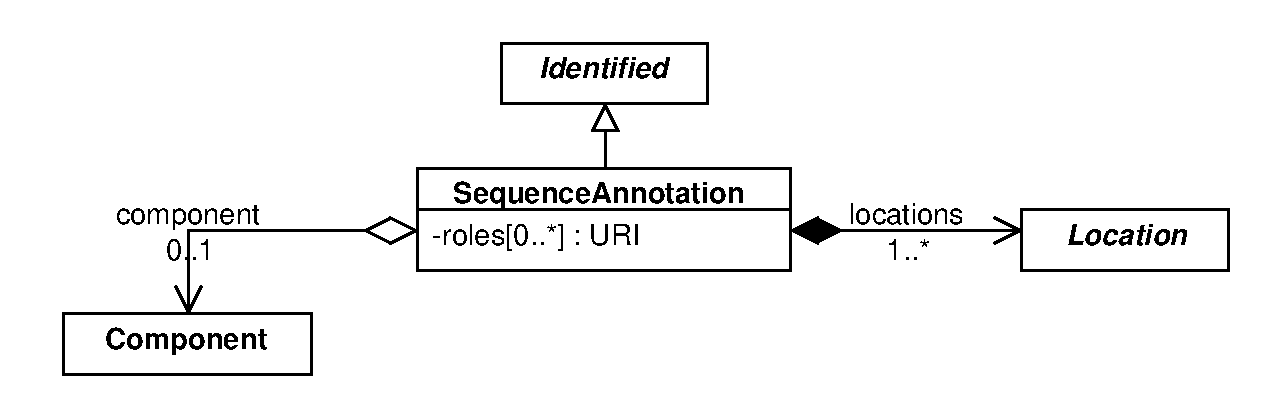
\includegraphics[scale=0.6]{uml/sequence_annotation}
\caption[]{Diagram of the \sbol{SequenceAnnotation} class and its associated properties.}
\label{uml:sequence_annotation}
\end{center}
\end{figure}

\paragraph{The \sbolheading{locations} property}\label{sec:locations}
\label{sec:locations}
The \sbol{locations} property is a REQUIRED set of one or more \sbol{Location} objects that indicate which \sbol{elements} of a \sbol{Sequence} are described by the \sbol{SequenceAnnotation}. 

In general, these \sbol{Location} objects SHOULD NOT cover the same \sbol{Sequence} \sbol{elements}.

\paragraph{The \sbolheading{component} property}\label{sec:component}
The \sbol{component} property is OPTIONAL and has a data type of \external{URI}. This \external{URI} MUST refer to a \sbol{Component} that is contained by the same parent \sbol{ComponentDefinition} that contains the \sbol{SequenceAnnotation}. In this way, the properties of the \sbol{SequenceAnnotation}, such as its \sbol{description} and \sbol{locations}, are associated with part of its parent \sbol{ComponentDefinition}'s substructure.

If the \sbol{SequenceAnnotation} contains a \sbol{Range} or \sbol{Cut} \sbol{Location} (see \ref{sec:Location}), then any \sbol{Component} it refers to MUST have a \sbol{ComponentDefinition} that refers to a \sbol{Sequence} with an \external{IUPAC} \sbol{encoding} from \ref{tbl:sequence_encodings}. 

\paragraph{Serialization}

The serialization of a \sbol{SequenceAnnotation} MUST have the form below. In this template, {\tt A\_LOCATION\_SUBCLASS} represents one of the \sbol{Location} subclasses.
\lstsetsbol
\begin{lstlisting}
<sbol:SequenceAnnotation rdf:about="...">
               ...   
  [\emph{zero or one}] <sbol:component rdf:resource="..."/> [\emph{element}] 
  [\emph{one}]         <sbol:location>
                 <sbol:A_LOCATION_SUBCLASS rdf:about="...">...</sbol:A_LOCATION_SUBCLASS>
               </sbol:location> [\emph{element}] 
</sbol:SequenceAnnotation>
\end{lstlisting}

The example below shows the serialization of a \sbol{SequenceAnnotation} object. It specifies the location of a particular \sbol{Component} named BBa\_F2620.
\lstsetsbol
\begin{lstlisting}
<sbol:SequenceAnnotation rdf:about="http://partsregistry.org/cd/BBa_F2620/anno2">
  <sbol:persistentIdentity rdf:resource="http://partsregistry.org/cd/BBa_F2620/anno2"/>
  <sbol:displayId>anno2</sbol:displayId>
  <sbol:location>
    <sbol:Range rdf:about="http://partsregistry.org/cd/BBa_F2620/anno2/range">
      <sbol:persistentIdentity rdf:resource="http://partsregistry.org/cd/BBa_F2620/anno2/range"/>
      <sbol:displayId>range</sbol:displayId>
      <sbol:start>56</sbol:start>
      <sbol:end>68</sbol:end>
      <sbol:orientation rdf:resource="http://sbols.org/v2#inline"/>
    </sbol:Range>
  </sbol:location>
  <sbol:component rdf:resource="http://partsregistry.org/cd/BBa_F2620/rbs"/>
</sbol:SequenceAnnotation>      
\end{lstlisting}

\subsubsection{Location}
\label{sec:Location}
The Location class is extended by the \sbol{Range}, \sbol{Cut}, and \sbol{GenericLocation} classes.  All of these thus share its \sbol{orientation} property, for example to to specify directionality on a potentially double-stranded \sbol{Component} object.

\begin{figure}[ht]
\begin{center}
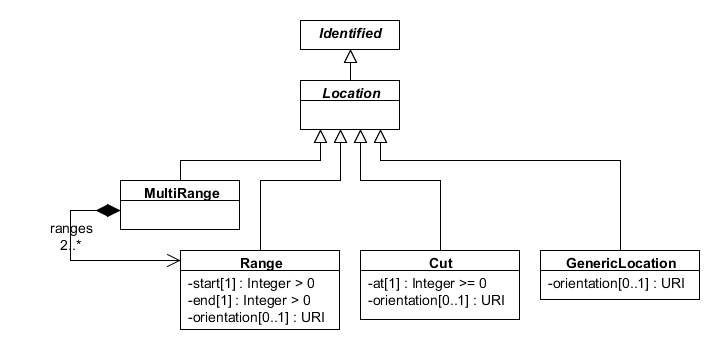
\includegraphics[scale=0.6]{uml/location}
\caption[]{Diagram of the \sbol{Location} class and its associated properties.}
\label{uml:location}
\end{center}
\end{figure}

\subparagraph{The \sbolheading{orientation} property}
\label{sec:orientation}

This OPTIONAL property has a URI value. For \sbol{ComponentDefinition} objects representing DNA molecules, it is RECOMMENDED to use one of the values in \ref{tbl:orientation_types}. 

\begin{table}[ht]
  \begin{edtable}{tabular}{l}
    \toprule
    \textbf{Orientation Types}  \\
    \midrule
    http://sbols.org/v2\#inline\\
    http://sbols.org/v2\#reverseComplement\\
    \bottomrule
  \end{edtable}
  \caption{URI constants for \sbol{orientation} values}
  \label{tbl:orientation_types}
\end{table}


\paragraph{Range}
\label{sec:Range}
A \sbol{Range} object specifies inclusive start and end positions. These properties are required in \sbol{Range} objects and they can have \external{integer} values greater than zero.

\subparagraph{The \sbolheading{start} property}\label{sec:start}
Specifies the start of a \sbol{Range}. This property is REQUIRED and can have \external{integer} values greater than zero.

\subparagraph{The \sbolheading{end} property}\label{sec:end}
Specifies the end of a \sbol{Range}. This property is REQUIRED and can have \external{integer} values greater than zero.

\subparagraph{Serialization}

The serialization of Range objects has the following form:
\lstsetsbol
\begin{lstlisting}
<sbol:Range rdf:about="...">
               ...   
  [\emph{one}]         <sbol:start>...</sbol:start> [\emph{element}] 
  [\emph{one}]         <sbol:end>...</sbol:end> [\emph{element}] 
  [\emph{zero or one}] <sbol:orientation rdf:resource="..."/> [\emph{element}] 
</sbol:Range>
\end{lstlisting}

The example below shows the serialization of a \sbol{Range} object. It specifies the region between 56 and 68, and the orientation is given as \external{inline}.
\lstsetsbol
\begin{lstlisting}
<sbol:Range rdf:about="http://partsregistry.org/cd/BBa_F2620/anno2/range">
  <sbol:persistentIdentity rdf:resource="http://partsregistry.org/cd/BBa_F2620/anno2/range"/>
  <sbol:displayId>range</sbol:displayId>
  <sbol:start>56</sbol:start>
  <sbol:end>68</sbol:end>
  <sbol:orientation rdf:resource="http://sbols.org/v2#inline"/>
</sbol:Range>
\end{lstlisting}

\paragraph{Cut}
\label{sec:Cut}
The \sbol{Cut} class has been introduced to enable the specification of a location between two indices. 
Each \sbol{Cut} object has the property \sbol{at}.

\subparagraph{The \sbolheading{at} property}
\label{sec:at}
The REQUIRED \sbol{at} property is an index greater than or equal to zero that specifies the index just before the location represented by the Cut object. 
A Cut object with \sbol{at} equal to zero represents the location just before index one (even though there is no zero index on Structure objects in SBOL). 

\subparagraph{Serialization}

The serialization of \sbol{Cut} objects has the following form:
\lstsetsbol
\begin{lstlisting}
<sbol:Cut rdf:about="...">
               ...   
  [\emph{one}]         <sbol:at>...</sbol:at> [\emph{element}] 
  [\emph{zero or one}] <sbol:orientation rdf:resource="..."/> [\emph{element}] 
</sbol:Cut>
\end{lstlisting}

The example below shows the serialization of a \sbol{Cut} object. It specifies the location after 27, and the orientation is given as \external{inline}.
\lstsetsbol
\begin{lstlisting}
<sbol:Cut rdf:about="http://partsregistry.org/cd/BBa_J23119/cutat10/cut">
  <sbol:persistentIdentity rdf:resource="http://partsregistry.org/cd/BBa_J23119/cutat10/cut"/>
  <sbol:displayId>cut</sbol:displayId>
  <sbol:at>10</sbol:at>
  <sbol:orientation rdf:resource="http://sbols.org/v2#inline"/>
</sbol:Cut>
\end{lstlisting}


\paragraph{GenericLocation}
\label{sec:GenericLocation}

While the \sbol{Range} and \sbol{Cut} classes are best suited to
describing locations on sequential structures, the
\sbol{GenericLocation} is included as a hook for extensions, e.g., for
describing locations in non-sequential structures.

\subparagraph{Serialization}

The serialization of \sbol{GenericLocation} objects has the following form:
\lstsetsbol
\begin{lstlisting}
<sbol:GenericLocation rdf:about="...">
               ...   
  [\emph{zero or one}] <sbol:orientation rdf:resource="..."/> [\emph{element}] 
</sbol:GenericLocation>
\end{lstlisting}

The example below shows the serialization of a \sbol{GenericLocation} object with a reverse orientation:
\lstsetsbol
\begin{lstlisting}
<sbol:GenericLocation rdf:about="http://www.partsregistry.org/Part:BBa_F2620/anno5/location">
  <sbol:orientation rdf:resource="http://sbols.org/v2#reverseComplement"/>
</sbol:GenericLocation>
\end{lstlisting}

\subsubsection{SequenceConstraint}
\label{sec:SequenceConstraint}
A \sbol{ComponentDefinition} object can link to \sbol{SequenceConstraint} objects to assert various kinds of structural restrictions between two \sbol{Component} objects that are its subcomponents. 
The purpose of \sbol{SequenceConstraint} is to allow partial designs to be specified when the precise identity, location, or ordering of \sbol{Component} objects is not yet fully determined.

A \sbol{SequenceConstraint} object requires \sbol{restriction}, \sbol{subject} and \sbol{object} properties to specify such constraints.

\begin{figure}[ht]
\begin{center}
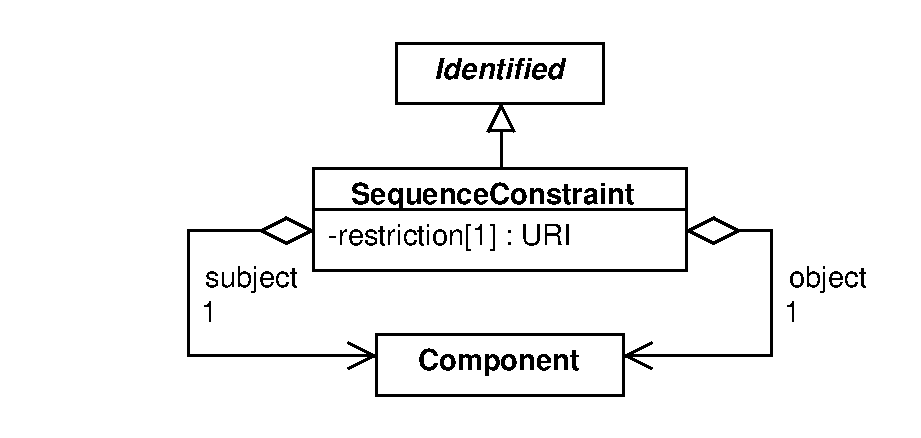
\includegraphics[scale=0.6]{uml/sequence_constraint}
\caption[]{Diagram of the \sbol{SequenceConstraint} class and its associated properties.}
\label{uml:sequence_constraint}
\end{center}
\end{figure}

\paragraph{The \sbolheading{subject} property}\label{sec:subject}
\label{sec:subject}
This REQUIRED property specifies the URI of the first \sbol{Component} object in the relation.

\paragraph{The \sbolheading{object} property}\label{sec:object}
\label{sec:object}
This REQUIRED property specifies the URI of the second \sbol{Component} object in the relation.

\paragraph{The \sbolheading{restriction} property}\label{sec:restriction}
\label{sec:restriction}

This REQUIRED property specifies a URI that identifies the type of relationship between the \sbol{subject} and \sbol{object} \sbol{Component} objects. 
The RECOMMENDED values for this property are given in \ref{tbl:restriction_types}.

Note: With regards to SBOL Version 1.1., this is a generalization of former \sbol{SequenceAnnotation} property \external{precedes}.

\begin{table}[ht]
  \begin{edtable}{tabular}{ll}
    \toprule
    \textbf{Restriction Types} & Subject/Object Relation \\
    \midrule
    http://sbols.org/v2\#precedes & Subject location is strictly less than object location \\
    http://sbols.org/v2\#sameOrientationAs & Subject and object have equal orientation URIs\\
    http://sbols.org/v2\#oppositeOrientationAs & Object orientation is ``opposite'' of subject\\    
    \bottomrule
  \end{edtable}
  \caption{URI constants for \sbol{restriction} values}
  \label{tbl:restriction_types}
\end{table}

\NVtodo{We need things like nextTo and overlapping, and think we might be able to get it from region-connection-calculus ontology}

\paragraph{Serialization}

The serialization of \sbol{SequenceConstraint} objects has the following form:
\lstsetsbol
\begin{lstlisting}
<sbol:SequenceConstraint rdf:about="...">
      ...
  [\emph{one}] <sbol:restriction rdf:resource="..."/> [\emph{element}]
  [\emph{one}] <sbol:subject rdf:resource="..."/> [\emph{element}]
  [\emph{one}] <sbol:object rdf:resource="..."/> [\emph{element}]
</sbol:SequenceConstraint>
\end{lstlisting}

The example below shows the serialization of a \sbol{SequenceConstraint} object. In the example, the constraint is included as part of a \sbol{ComponentDefinition} for a LacI repressible composite promoter and has a precedes restriction. This restriction states that the subject \sbol{Component} for the core promoter precedes the object \sbol{Component} for the LacI operator in the composite promoter definition. Such restriction is especially useful to specify incomplete designs and the final design may include other components between the subject and object components. 
\lstsetsbol
\begin{lstlisting}
<sbol:SequenceConstraint rdf:about="http://partsregistry.org/cd/BBa_K174004/r1">
  <sbol:persistentIdentity rdf:resource="http://partsregistry.org/cd/BBa_K174004/r1"/>
  <sbol:displayId>r1</sbol:displayId>
  <sbol:restriction rdf:resource="http://sbols.org/v2#precedes"/>
  <sbol:subject rdf:resource="http://partsregistry.org/cd/pspac"/>
  <sbol:object rdf:resource="http://partsregistry.org/cd/LacI_operator"/>
</sbol:SequenceConstraint>
\end{lstlisting}

\subsection{Model}
\label{sec:Model}

\begin{figure}[ht]
\begin{center}
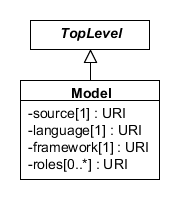
\includegraphics[scale=0.6]{uml/model}
\caption[]{Diagram of the \sbol{Model} class and its associated properties.}
\label{uml:model}
\end{center}
\end{figure}

SBOL's \sbol{Model} objects are placeholders that point to some external modeling mechanism, with some additional meta-data to enable better reasoning about the contents of that external mechanism.
In this way, there is minimal duplication of standardization efforts and users of SBOL can specify the quantitative function of \sbol{ModuleDefinition} objects in a well-developed language of their choice. 

Each \sbol{Model} object specifies the location of the actual content of a qualitative/quantitative model, the language the model is implemented with, the modeling framework and the model's role(s). 

\subsubsection*{ The \sbolheading{source} property}\label{sec:source}
This REQUIRED property is a URI that specifies the actual location of a qualitative or quantitative model.

\subsubsection*{ The \sbolheading{language} property}\label{sec:language}
This REQUIRED property is a URI that specifies the language the model is implemented with. 
Values for this URI are RECOMMENDED to be chosen from the EMBRACE Data and Methods (EDAM) ontology where possible. A few suggested model types and corresponding URI values are shown in \ref{tbl:model_types}.

\begin{table}[ht]
  \begin{edtable}{tabular}{ll}
    \toprule
    \textbf{Model Language} & \textbf{URI} \\
    \midrule
    SBML  & \url{http://identifiers.org/edam/format_2585}\\
    CellML		 & \url{http://identifiers.org/edam/format_3240}\\
    BioPAX    & \url{http://identifiers.org/edam/format_3156}\\
    \bottomrule
  \end{edtable}
  \caption{Some commonly used model languages and their corresponding URIs.}
  \label{tbl:model_types}
\end{table}


\subsubsection*{ The \sbolheading{framework} property}\label{sec:framework}
This REQUIRED property is a URI that specifies the modeling framework that a model is implemented within. 
Values for this URI are RECOMMENDED to be chosen from the SBO's modeling framework terms where possible. A few suggested model frameworks and corresponding URI values are shown in \ref{tbl:model_frameworks}.

\begin{table}[ht]
  \begin{edtable}{tabular}{ll}
    \toprule
    \textbf{Framework} & \textbf{URI} \\
    \midrule
    Continuous  & \url{http://identifiers.org/biomodels.sbo/SBO:0000062}\\
    Discrete & \url{http://identifiers.org/biomodels.sbo/SBO:0000063}\\
    \bottomrule
  \end{edtable}
  \caption{Example modelling frameworks and corresponding SBO terms.}
  \label{tbl:model_frameworks}
\end{table}

\subsubsection*{Serialization}

The serialization of \sbol{Model} objects has the following form:

\lstsetsbol
\begin{lstlisting}
<sbol:Model rdf:about="http://www.sbolstandard.org/examples/toogleswicth">
      ...
  [\emph{one}] <sbol:source rdf:resource="..."/> [\emph{element}]
  [\emph{one}] <sbol:language rdf:resource="..."/> [\emph{element}]
  [\emph{one}] <sbol:framework rdf:resource="..."/> [\emph{element}]
</sbol:Model>
\end{lstlisting}

The example below shows the serialization of a \sbol{Model} object. The model object includes information about the models of a toggle switch. The model is implemented in SBML using a continuous modelling framework. The source property shows the physical location of the SBML model, in a model repository. 
\lstsetsbol
\begin{lstlisting}
<?xml version="1.0" ?>
<rdf:RDF xmlns:rdf="http://www.w3.org/1999/02/22-rdf-syntax-ns#" xmlns:dcterms="http://purl.org/dc/terms/" xmlns:prov="http://www.w3.org/ns/prov#" xmlns:sbol="http://sbols.org/v2#">
  <sbol:Model rdf:about="http://www.sbolstandard.org/examples/pIKE_Toggle_1">
    <sbol:persistentIdentity rdf:resource="http://www.sbolstandard.org/examples/pIKE_Toggle_1"/>
    <sbol:displayId>pIKE_Toggle_1</sbol:displayId>
    <dcterms:title>pIKE_Toggle_1 toggle switch</dcterms:title>
    <sbol:source rdf:resource="http://virtualparts.org/part/pIKE_Toggle_1"/>
    <sbol:language rdf:resource="http://identifiers.org/edam/format_2585"/>
    <sbol:framework rdf:resource="http://identifiers.org/biomodels.sbo/SBO:0000062"/>
  </sbol:Model>
</rdf:RDF>
\end{lstlisting}
\label{ser:Model}

\subsection{ModuleDefinition}
\label{sec:ModuleDefinition}

\begin{figure}[ht]
\begin{center}
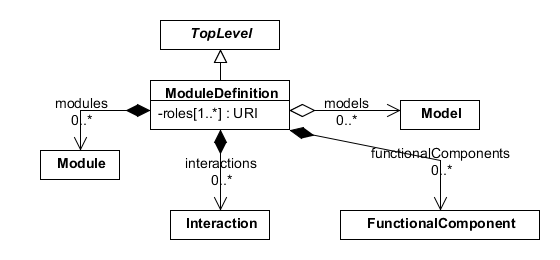
\includegraphics[scale=0.6]{uml/module_definition}
\caption[]{Diagram of the \sbol{ModuleDefinition} class and its associated properties.}
\label{uml:module_definition}
\end{center}
\end{figure}

The \sbol{ModuleDefinition} class is the hub where the structural and functional aspects of genetic designs are brought together to form a complete picture of the design. 
A \sbol{ModuleDefinition} object is composed from zero or more \sbol{FunctionalComponent}, \sbol{Module}, and \sbol{Interaction} objects, and links to zero or more \sbol{Model} objects. 

As an engineering object, a \sbol{ModuleDefinition} will often have certain of its \sbol{FunctionalComponent} objects that are intended to carry signals in or out of it.  
This functionality of designated ``inputs'' and ``outputs'' is expressed by \sbol{direction} properties on its \sbol{FunctionalComponent} elements.

\subsubsection*{The \sbolheading{roles} property}\label{sec:roles}
The \sbol{roles} property is an OPTIONAL set of \external{URI}s that clarifies the intended function of a \sbol{ModuleDefinition} in a biological context.  

These terms might identify ``logical'' roles, such as ``inverter'' or ``AND gate'', or they might identify descriptive biological roles, such as ``metabolic pathway'' and ``signaling cascade,'' or might identify roles from some other manner of describing intended function.

\subsubsection*{The \sbolheading{modules} property}\label{sec:modules}

The \sbol{modules} property is OPTIONAL and MAY specify a set of \sbol{Module} objects contained by the \sbol{ModuleDefinition}.

While the \sbol{ModuleDefinition} class is analogous to a blueprint or specification sheet for a system of interaction biological elements, the \sbol{Module} class represents the specific occurrence of a particular sub-system within that design. Hence, this class allows a biological design to include multiple copies of a subsystem. For example, the \sbol{ModuleDefinition} for a network of two-input repressor systems, where the particular repressors have not yet been chosen, contain multiple \sbol{Module} objects that refer to the same \external{URI} for the \sbol{ModuleDefinition} of an abstract two-input repressor device.

\subsubsection*{The \sbolheading{functionalComponents} property}
\label{sec:functionalComponents}

The \sbol{functionalComponents} property is OPTIONAL and MAY specify a set of \sbol{FunctionalComponent} objects contained by the \sbol{ModuleDefinition}.

Just as a \sbol{Module} represents an instance of a subsystem in the ``blueprint'' of a \sbol{ModuleDefinition}, a \sbol{FunctionalComponent} represents an instance of an individual element whose \sbol{ComponentDefinition} may be used multiple times in a \sbol{ModuleDefinition}.  For example, a \sbol{ModuleDefinition} might contain several copies of a particular promoter.

\subsubsection*{The \sbolheading{interactions} property}\label{sec:interactions}

The \sbol{interactions} property is OPTIONAL and MAY specify a set of \sbol{Interaction} objects contained by the \sbol{ModuleDefinition}.

The \sbol{Interaction} class provides an abstract, machine-friendly representation of the functional interactions of entities within a \sbol{ModuleDefinition} (whereas a \sbol{Model} is concrete and may not be readily susceptible to machine reasoning, depending on how it is implemented).  Each \sbol{Interaction} includes \sbol{Participation} entities that indicate the roles of the \sbol{FunctionalComponent} objects involved in the \sbol{Interaction}

\subsubsection*{The \sbolheading{models} property}\label{sec:models}
The \sbol{models} property is OPTIONAL and MAY specify a set of \external{URI}s identifying \sbol{Model} objects.

SBOL's \sbol{Model} objects are placeholders used to link specifications of biological parts and their interactions to computational models of arbitrary format.
A \sbol{ModuleDefinition} object can link to more than one \sbol{Model} since each might encode the same system in a different way or at a different level of detail.

\subsubsection*{Serialization}

The serialization of \sbol{ModuleDefinition} has the following form:
\lstsetsbol
\begin{lstlisting}
<sbol:ModuleDefinition rdf:about="...">
               ...
  [\emph{zero or more}]  <sbol:role rdf:resource="..."/> [\emph{elements}]
  [\emph{zero or more}]  <sbol:model rdf:resource="..."/> [\emph{elements}]
  [\emph{zero or more}] <sbol:functionalComponent>
                 <sbol:FunctionalComponent rdf:about="...">...</sbol:FunctionalComponent >
               </sbol:functionalComponent> [\emph{elements}]
  [\emph{zero or more}] <sbol:module>
                 <sbol:Module rdf:about="...">...</sbol:Module>
               </sbol:module> [\emph{elements}]
  [\emph{zero or more}] <sbol:interaction>
                 <sbol:Interaction rdf:about="...">...</sbol:Interaction>
               </sbol:interaction> [\emph{elements}]
</sbol:ModuleDefinition>
\end{lstlisting}

The example below shows a simple \sbol{ModuleDefinition} containing two components, a \sbol{FunctionalComponent} for a DNA sequence encoding constitutive expression of GFP and another for the GFP protein expressed from this sequence, plus an interaction describing that relation.

\lstsetsbol
\begin{lstlisting}
<sbol:ModuleDefinition rdf:about="http://sbolstandard.org/example/md/GFP_expression">
  <sbol:functionalComponent>
    <sbol:FunctionalComponent rdf:about="http://sbolstandard.org/example/md/GFP_expression/GFP_protein">
      <sbol:definition rdf:resource="http://sbolstandard.org/example/GFP"/>
      <sbol:access rdf:resource="http://sbols.org/v2#public"/>
      <sbol:direction rdf:resource="http://sbols.org/v2#output"/>
    </sbol:FunctionalComponent>
  </sbol:functionalComponent>
  <sbol:functionalComponent>
    <sbol:FunctionalComponent rdf:about="http://sbolstandard.org/example/md/GFP_expression/Constitutive_GFP">
      <sbol:definition rdf:resource="http://sbolstandard.org/example/GFP_generator"/>
      <sbol:access rdf:resource="http://sbols.org/v2#public"/>
      <sbol:direction rdf:resource="http://sbols.org/v2#none"/>
    </sbol:FunctionalComponent>
  </sbol:functionalComponent>
  <sbol:interaction>
    <sbol:Interaction rdf:about="http://sbolstandard.org/example/md/GFP_expression/express_GFP">
      ...
    </sbol:Interaction>
  </sbol:interaction>
</sbol:ModuleDefinition>
\end{lstlisting}

\subsubsection{FunctionalComponent}
\label{sec:FunctionalComponent}
A \sbol{FunctionalComponent} is an instance of a \sbol{ComponentDefinition} being used as part of a \sbol{ModuleDefinition}
Each FunctionalComponent object is owned by a \sbol{ModuleDefinition} and serves as an explicit usage of a \sbol{ComponentDefinition} object for the purpose of fulfilling some function. 

\sbol{FunctionalComponent} derives from \sbol{ComponentInstance}, and therefore has the \sbol{definition}, \sbol{access}, and \sbol{mapsTos} properties. 
Additionally, it has a \sbol{direction} property that specifies whether it serves as an input, output, both, or neither with regards to the \sbol{ModuleDefinition} that contains it.

\paragraph{The \sbolheading{direction} property}\label{sec:direction}
Each \sbol{FunctionalComponent} MUST specify via the \sbol{direction} property whether it serves as an  input, output, both, or neither for its parent \sbol{ModuleDefinition} object. 
The value for this property MUST be one of the values given in \ref{tbl:functionalcomponent_directions}.


\begin{table}[ht]
  \begin{edtable}{tabular}{ll}
    \toprule
    \textbf{Direction URI} & \textbf{Description} \\
    \midrule
    \url{http://sbols.org/v2#inout}  & To indicate a \sbol{FunctionalComponent} can be used as both input or output\\
    \url{http://sbols.org/v2#in}  & To indicate a \sbol{FunctionalComponent} can be used as input\\
    \url{http://sbols.org/v2#out}  & To indicate a \sbol{FunctionalComponent} can be used as output\\
    \url{http://sbols.org/v2#none}  & To indicate a \sbol{FunctionalComponent} is neither input nor output\\
    \bottomrule
  \end{edtable}
  \caption{URIs for the \sbol{direction} property.}
  \label{tbl:functionalcomponent_directions}
\end{table}

The purpose of \sbol{direction} is to encode a common way in which designers think about the ``purpose'' of a \sbol{FunctionalComponent} within a \sbol{ModuleDefinition}.
For example, consider a system that is designed to indicate concentration of the cell-cell signalling molecule 3OC$_6$HSL by the concentration of the product of a particular CDS.
In this system, the concentration of 3OC$_6$HSL is the signal being interpreted by the system, so the \sbol{FunctionalComponent} for 3OC$_6$HSL would have a \sbol{direction} of ``input.''  
Complementarily, the concentration of the designated product is the signal intended for consumption by other biologicals systems, and so the \sbol{FunctionalComponent} for that product would have a \sbol{direction} of ``output.''
The CDS encoding the product, however, is not intended to interact directly, and so its \sbol{FunctionalComponent} would have a \sbol{direction} of ``neither.''
Finally, in some cases a \sbol{FunctionalComponent} may serve as both an input and output, and be marked as having a \sbol{direction} of ``both.''

\paragraph{Serialization}

The serialization of \sbol{FunctionalComponent}s has the following form.
\lstsetsbol
\begin{lstlisting}
<sbol:FunctionalComponent rdf:about="...">
               ...
  [\emph{one}]          <sbol:definition rdf:resource="..."/> [\emph{element}]
  [\emph{one}]          <sbol:access rdf:resource="..."/> [\emph{element}]
  [\emph{one}]          <sbol:direction rdf:resource="..."/> [\emph{element}]
  [\emph{zero or more}] <sbol:mapsTo rdf:resource="..."/> [\emph{elements}]
</sbol:FunctionalComponent>
\end{lstlisting}

In the example below, the functional component is defined as public input or output. The component refers to the \texttt{Part:BBa\_R0010} promoter from the Parts Registry.
\lstsetsbol
\begin{lstlisting}
<sbol:FunctionalComponent rdf:about="http://sbolstandard.org/example/laci_inverter/promoter">
  <sbol:definition rdf:resource="http://www.partsregistry.org/BBa_R0010"/>
  <sbol:access rdf:resource="http://sbols.org/v2#public"/>
  <sbol:direction rdf:resource="http://sbols.org/v2#inout"/>
</sbol:FunctionalComponent>
\end{lstlisting}

\subsubsection{Module}
\label{sec:Module}

\begin{figure}[ht]
\begin{center}
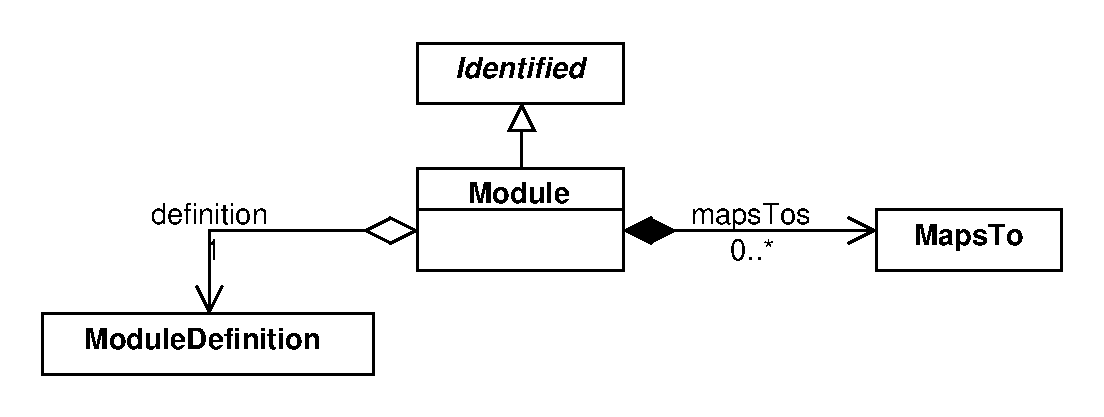
\includegraphics[scale=0.6]{uml/module}
\caption[]{Diagram of the \sbol{Module} class and its associated properties.}
\label{uml:module}
\end{center}
\end{figure}

The \sbol{Module} class represents the usage or occurrence of a \sbol{ModuleDefinition} within a larger design (that is, another \sbol{ModuleDefinition}).  

\paragraph{The \sbolheading{definition} property}
\label{sec:definition}

The \sbol{definition} property is a REQUIRED \external{URI} that refers to the \sbol{ModuleDefinition} for the \sbol{Module}.

The \sbol{definition} property MUST NOT refer to the same \sbol{ModuleDefinition} as that which contains the \sbol{Module}. Furthermore, \sbol{Module} objects MUST NOT form a circular chain of references via their \sbol{definition} properties and the \sbol{ModuleDefinition} objects that contain them. For example, consider the \sbol{Module} objects $A$ and $B$ and the \sbol{ModuleDefinition} objects $X$ and $Y$. The reference chain ``$X$ contains $A$, $A$ is defined by $Y$, $Y$ contains $B$, and $B$ is defined by $X$'' is circular. 

\paragraph{The \sbolheading{mapsTo} property}
\label{sec:mapsTos}

The \sbol{mapsTos} property is an OPTIONAL set of \sbol{MapsTo} objects that refer to and link \sbol{Module} objects together within a larger design.

\ref{sec:MapsTo} contains a detailed description of the \sbol{MapsTo} class.

\paragraph{Serialization}
The serialization of \sbol{Module}s has the following form.
\lstsetsbol
\begin{lstlisting}
<sbol:Module rdf:about="...">
  [\emph{one}]          <sbol:definition rdf:resource="..."/> [\emph{element}]
  [\emph{zero or more}] <sbol:mapsTo>
                 <sbol:MapsTo rdf:about="...">...</sbol:MapsTo>
               </sbol:mapsTo> [\emph{element}]
</sbol:Module>
\end{lstlisting}

The example below specifies a TetR inverter that is being used as
a part of a toggle switch:

\lstsetsbol
\begin{lstlisting}
<sbol:Module rdf:about="http://sbolstandard.org/example/toggle_switch/tetr_inverter">
  <sbol:definition rdf:resource="http://sbolstandard.org/example/tetr_inverter"/>
  ...
</sbol:Module>
\end{lstlisting}

\subsubsection{Interaction}
\label{sec:Interaction}

\begin{figure}[ht]
\begin{center}
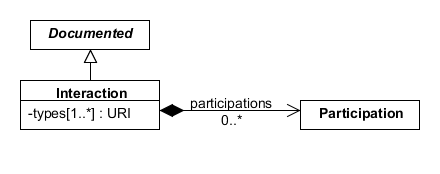
\includegraphics[scale=0.6]{uml/interaction}
\caption[]{Diagram of the \sbol{Interaction} class and its associated properties.}
\label{uml:interaction}
\end{center}
\end{figure}

The \sbol{Interaction} class provides a description of the functional interactions of entities within a \sbol{ModuleDefinition}.
For example, it can be used to represent regulatory interactions, such as activation or repression, processes from the central dogma of biology, such as transcription and translation, or molecular interactions like  non-covalent binding between a small molecule and transcription factor or phosphorylation of a transcription factor by an enzyme.
Such an \sbol{Interaction} is represented in SBOL by referring to an ontology defining the type of interaction and declaring how various entities participate in the interaction.

\paragraph{The \sbolheading{types} property}\label{sec:types}

The \sbol{types} property is a REQUIRED set of one or more URIs that identify an appropriate ontology term describing the behavior represented by this \sbol{Interaction}. 
If an \sbol{Interaction} object has multiple
\sbol{types} URIs, then they must identify synonymous terms.

Values for this URI are RECOMMENDED to be chosen from the occurring entity relationship branch of the Systems Biology Ontology (SBO), where possible.

\paragraph{The \sbolheading{participations} property}\label{sec:participations}

The \sbol{participations} property is an OPTIONAL set of \sbol{Participation} objects, each of which identifies a \sbol{FunctionalComponent} and the \sbol{roles} it plays in the interaction.


\paragraph{Serialization}

The serialization of \sbol{Interaction} objects has the following form.
\lstsetsbol
\begin{lstlisting}
<sbol:Interaction rdf:about="...">
               ...  
  [\emph{one or more}]  <sbol:type rdf:resource="..."/> [\emph{elements}]
  [\emph{zero or more}] <sbol:participation>
                 <sbol:Participation rdf:about="...">...</sbol:Participation>
               </sbol:participation> [\emph{elements}]
</sbol:Interaction>
\end{lstlisting}

The example below shows an \sbol{Interaction} representing an inhibition relationship between a repressor and a promoter (omitting the details of the \sbol{Participation} objects):

\lstsetsbol
\begin{lstlisting}
<sbol:Interaction rdf:about="http://sbolstandard.org/example/laci_inverter/LacI_pLacI">
  <sbol:type rdf:resource="http://identifiers.org/biomodels.sbo/SBO:0000169"/>
  <sbol:participation>
    <sbol:Participation rdf:about="...">
	  ... 	
    </sbol:Participation>
  </sbol:participation>
  <sbol:participation>
    <sbol:Participation rdf:about="...">
      ... 
    </sbol:Participation>
  </sbol:participation>
</sbol:Interaction>
\end{lstlisting}


\begin{figure}[ht]
\begin{center}
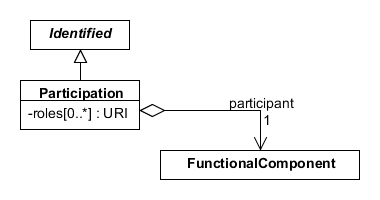
\includegraphics[scale=0.6]{uml/participation}
\caption[]{Diagram of the \sbol{Participation} class and its associated properties.}
\label{uml:participation}
\end{center}
\end{figure}

\subsubsection{Participation}
\label{sec:Participation}

Each \sbol{Participation} object describes the role or roles that a
particular \sbol{FunctionalComponent} plays in its parent
\sbol{Interaction}.

\paragraph{The \sbolheading{roles} property}\label{sec:roles}

The \sbol{roles} property is an OPTIONAL set of URIs that identify an appropriate ontology term describing this elements relationship to its parent \sbol{Interaction}. 
If a \sbol{Participation} object has multiple
\sbol{roles} URIs, then they must identify synonymous terms.

Values for this URI are RECOMMENDED to be chosen from the participant role branch of the Systems Biology Ontology (SBO) where possible.

\paragraph{The \sbolheading{participant} property}\label{sec:participant}

The \sbol{participant} property MUST specify precisely one \sbol{FunctionalComponent} object that plays the designated \sbol{roles} in its parent \sbol{Interaction} object.


\paragraph{Serialization}

The serialization of \sbol{Participation} objects has the following form.
\lstsetsbol
\begin{lstlisting}
<sbol:Participation rdf:about="...">
               ...
  [\emph{zero or more}] <sbol:role rdf:resource="..."/> [\emph{elements}]
  [\emph{one}]          <sbol:participant rdf:resource="..."/> [\emph{element}]
</sbol:Participation>
\end{lstlisting}

In the example below, the role of participating \sbol{FunctionalComponent} is defined to be \external{inhibitor}, using the \external{SBO:0000020} term. This component is specified using the participant property of the \sbol{Participation} entity.
\lstsetsbol
\begin{lstlisting}
<sbol:Participation rdf:about="http://sbolstandard.org/example/laci_inverter/LacI_pLacI/P03023">
  <sbol:role rdf:resource="http://identifiers.org/biomodels.sbo/SBO:0000020"/>
  <sbol:participant rdf:resource="http://sbolstandard.org/example/laci_inverter/TF"/>
</sbol:Participation>
\end{lstlisting}

\subsection {Collection}
\label{sec:Collection}
The \sbol{Collection} class is a class that groups together a set of \sbol{TopLevel} objects that have something in common. 
Some examples of \sbol{Collection} objects:
\begin{itemize}
\item Results of a query to find all \sbol{ComponentDefinition} objects that function as promoters in a repository.
\item A set of \sbol{ModuleDefinition} objects representing a library of NAND gates.
\item A \sbol{ModuleDefinition} for a complex design, and all of the \sbol{ModuleDefinition}, \sbol{ComponentDefinition}, \sbol{Sequence}, and \sbol{Model} objects used to provide its full specification.
\end{itemize}

\begin{figure}[ht]
\begin{center}
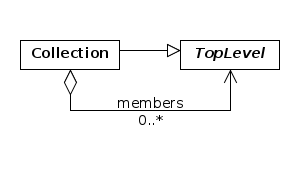
\includegraphics[scale=0.6]{uml/collection}
\caption[]{Diagram of the \sbol{Collection} class and its associated properties.}
\label{uml:collection}
\end{center}
\end{figure}

\subsubsection*{The \sbolheading{members} property}\label{sec:members}
The \sbol{members} property has a data type of URI and has the URI for a \sbol{TopLevel} entity.  A \sbol{Collection} may have any number of members, including none.

\subsubsection*{Serialization}

The serialization of \sbol{Collection} objects has the following form:

\lstsetsbol
\begin{lstlisting}
<sbol:Collection rdf:about="...">
               ...
  [\emph{zero or more}] <sbol:member rdf:resource="..."/> [\emph{element}]
</sbol:Collection>
\end{lstlisting}

The example below shows the serialization of a \sbol{Collection} object grouping together a library of constitutive promoters.
\lstsetsbol
\begin{lstlisting}
<?xml version="1.0" ?>
<rdf:RDF xmlns:rdf="http://www.w3.org/1999/02/22-rdf-syntax-ns#" xmlns:dcterms="http://purl.org/dc/terms/" xmlns:prov="http://www.w3.org/ns/prov#" xmlns:sbol="http://sbols.org/v2#">
  <sbol:Collection rdf:about="http://parts.igem.org/Promoters/Catalog/Anderson">
    <sbol:persistentIdentity rdf:resource="http://parts.igem.org/Promoters/Catalog/Anderson"/>
    <sbol:displayId>Anderson</sbol:displayId>
    <dcterms:title>Anderson promoters</dcterms:title>
    <dcterms:description>The Anderson promoter collection</dcterms:description>
    <sbol:member rdf:resource="http://partsregistry.org/Part:BBa_J23119"/>
    ...
    <sbol:member rdf:resource="http://partsregistry.org/Part:BBa_J23118"/>
  </sbol:Collection>
</rdf:RDF>
\end{lstlisting}
\label{ser:Collection}

\subsection{Extending the SBOL Representation:  Annotations}
\label{sec:Annotations}
\label{sec:annotations}

SBOL does not attempt to represent all information about a biological system, since many things do not yet have a clear ``right way'' to be represented, such as design intent, biological context, or performance data.  Instead, SBOL allows the embedding of application specific data that are not captured by the SBOL standard.  Such data are optional, but can be computationally generated and exchanged via SBOL documents without getting damaged or lost. 

To do this, SBOL provides an ``annotation'' mechanism for attaching arbitrary information to SBOL objects, which allows SBOL models to be connected with any other models in an extensible manner.
In particular, three methods are supported for connecting the SBOL data model with other, possibly application-specific data:
\begin{enumerate}
\item Information that is ``part'' of an SBOL object (i.e., a ``filled diamond'' relationship) is annotated simply by adding non-conflicting properties and custom entries to an SBOL object.  An example might be source information about the registry from which a \sbol{ComponentDefinition} was imported.
\item Information that is an independent object is annotated by wrapping it inside of a \sbol{GenericTopLevel} object.  An example might be a data sheet describing the performance of a \sbol{ModuleDefinition} in some particular context.
\item Conversely, rather than embedding external objects in SBOL, SBOL objects can also be linked to external data.  The only requirement is that some URI resolution mechanism must be available that allows the links from SBOL objects to be followed when needed.
\end{enumerate}

\subsubsection{Annotating SBOL objects}
% whole set of labels for the properties defined herein
\label{sec:value}
\label{sec:Annotation}
\label{sec:AnnotationValue}
\label{sec:NestedAnnotations}
\label{sec:nestedQName}
\label{sec:nestedURI}

Each \sbol{Identified} object may have a number of annotations in the form of name/value property pairs. The \sbol{name} property is specified by a qualified name (\external{QName}), which is composed of a namespace, a prefix, and a local name. The \sbol{value} property can be a literal type (i.e., \external{String}, \external{Integer}, \external{Double}, \external{Boolean}), \external{URI}, or a \sbol{NestedAnnotations} object. The \sbol{NestedAnnotations} object is composed of a \sbol{nestedQName}, \sbol{nestedURI}, and an optional list of nested \sbol{annotations}.

\Ctodo{NIC: Please update UML as follows: remove link from Identifed to AnnotationValue, change type of name to QName, add new class NestedAnnotations that inherits from AnnotationValue with properties nestedQName : QName, nestedURI : URI, and a 0..* annotations link to the Annotation class.}

\begin{figure}[!ht]
\begin{center}
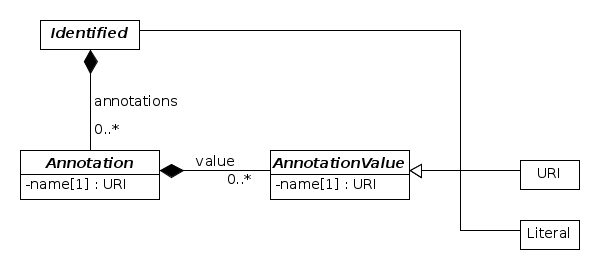
\includegraphics[scale=0.6]{uml/identified_annotations}
\caption[]{Diagram of the \sbol{Annotation} class and its association with \sbol{Identified} and \sbol{AnnotationValue} objects, which is used for annotating SBOL entities with application specific data.}
\label{uml:identified_annotations}
\end{center}
\end{figure}

\subsubsection*{Serialization}

The serialization of \sbol{Annotation} objects has the following form:

\lstsetsbol
\begin{lstlisting}
<?xml version="1.0" ?>
<rdf:RDF xmlns:rdf="http://www.w3.org/1999/02/22-rdf-syntax-ns#" 
  xmlns:sbol="http://sbols.org/v2#"
  xmlns:prefix1="NAMESPACE_1" 
  xmlns:prefix2="NAMESPACE_2" 
  xmlns:nestedObjectPrefix="A_NESTED_OBJECT_NAMESPACE" 
  ...
 >
<sbol:A_TOPLEVELOBJECT rdf:about="...">
                ...
  [\emph{zero or more}] <prefix1:LOCAL_NAME_1>A_LITERAL</prefix:LOCAL_NAME_1> [\emph{elements}]
  [\emph{zero or more}] <prefix1:LOCAL_NAME_2 rdf:resource=URI/> [\emph{elements}]
  [\emph{zero or more}] <prefix2:LOCAL_NAME_3>
                  <nestedObjectPrefix:NESTED_LOCAL_NAME rdf:about="...">
                    ...
                  </nestedObjectPrefix:NESTED_LOCAL_NAME>
                </prefix2:LOCAL_NAME_3> [\emph{elements}]
</sbol:TOPLEVELOBJECT>
\end{lstlisting}
The \sbol{name} property species the namespace, prefix, and localPart values.  The first form is for a \external{literal} annotation.  The second form is for a \external{URI} annotation.  Finally, the third form is for an \sbol{NestedAnnotations} object annotation.  In this last case, the \sbol{nestedQName} property specifies the nestedNamespace, nestedPrefix, and nestedLocalPart while the \sbol{nestedURI} property species the URI for the nested annotation.

The ComponentDefinition example for a promoter serialized below shows how annotations can be added to SBOL objects. Annotations are added using the relevant information from the Parts Registry. Annotation property names are qualified with the \external{http://www.partsregistry.org/} namespace, which is prefixed using \external{pr}. The first annotation is named as \external{pr:group}, indicating the iGEM group designing the promoter, and has a \external{String} value. The second \external{pr:experience} annotation has a \external{URI} value and is serialised as an RDF resource pointing to the information Web page on the Parts Registry for the promoter. The  \external{pr:information} property represents a complex annotation which is a type of \external{pr:Information} and includes information about the regulatory details of the promoter using Parts Registry categories.   

\begin{figure} [ht]
\lstsetsbol
\begin{lstlisting}
<?xml version="1.0" ?>
<rdf:RDF xmlns:pr="http://partsregistry.org" xmlns:rdf="http://www.w3.org/1999/02/22-rdf-syntax-ns#" xmlns:dcterms="http://purl.org/dc/terms/" xmlns:prov="http://www.w3.org/ns/prov#" xmlns:sbol="http://sbols.org/v2#">
  <sbol:ComponentDefinition rdf:about="http://partsregistry.org/cd/BBa_J23119">
    <sbol:persistentIdentity rdf:resource="http://partsregistry.org/cd/BBa_J23119"/>
    <sbol:displayId>BBa_J23119</sbol:displayId>
    <pr:group>iGEM2006_Berkeley</pr:group>
    <pr:experience rdf:resource="http://parts.igem.org/cgi/partsdb/part_info.cgi?part_name=BBa_J23119"/>
    <pr:information>
      <pr:Information rdf:about="http://parts.igem.org/cgi/partsdb/part_info.cgi?part_name=BBa_J23119">
        <pr:sigmafactor>//rnap/prokaryote/ecoli/sigma70</pr:sigmafactor>
        <pr:regulation>//regulation/constitutive</pr:regulation>
      </pr:Information>
    </pr:information>
    <dcterms:title>J23119</dcterms:title>
    <dcterms:description>Constitutive promoter</dcterms:description>
    <sbol:type rdf:resource="http://www.biopax.org/release/biopax-level3.owl#DnaRegion"/>
    <sbol:role rdf:resource="http://identifiers.org/so/SO:0000167"/>
  </sbol:ComponentDefinition>
</rdf:RDF>
\end{lstlisting}
\label{ser:Annotation}
\end{figure}

\subsubsection{GenericTopLevel}  
\label{sec:GenericTopLevel}

SBOL documents can also be annotated at the top level. 
SBOL's \sbol{GenericTopLevel} is a top-level entity whose only purpose is to include a set of annotations as described above. 
Entities that have independent existence (i.e., would be another ``top level'' class) and are not recognized by the SBOL standard are loaded into these top level entities. 
These \sbol{GenericTopLevel} entities can thus be safely used by tools to exchange non-SBOL data embedded separately within SBOL.
As with any other top level entities, \sbol{GenericTopLevel} entities may include SBOL properties such as \sbol{displayId}, \sbol{name}, \sbol{description}, etc. The type of data found in the generic entity is indicated using the \sbol{rdfType} property which is of type \external{QName}.   

\begin{figure}[ht]
\begin{center}
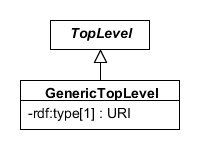
\includegraphics[scale=0.6]{uml/generictoplevel}
\caption[]{Diagram of the \sbol{GenericTopLevel} class and its associated properties, which is used for embedding externally defined entities into SBOL documents.}
\label{uml:generictoplevel}
\end{center}
\end{figure}

\subsubsection*{Serialization}

The serialization of \sbol{GenericTopLevel} objects has the following form where the prefix, namespace, and localPart are defined by the \sbol{rdfType} property:

%<?xml version="1.0" ?>
%<rdf:RDF ... xmlns:prefix=namespace ...>
%<prefix:localPart rdf:about="...">
%              ...
%</prefix:localPart>

\lstsetsbol
\begin{lstlisting}
<?xml version="1.0" ?>
<rdf:RDF xmlns:rdf="http://www.w3.org/1999/02/22-rdf-syntax-ns#" 
  xmlns:sbol="http://sbols.org/v2#"
  xmlns:applicationPrefix="APPLICATION_NAMESPACE" 
  ...
 >
<applicationPrefix:APPLICATION_OBJECT_NAME rdf:about="...">
  ...
</applicationPrefix:APPLICATION_OBJECT_NAME>
\end{lstlisting}

The example below shows how a datasheet object can be added to an SBOL document using the \sbol{GenericTopLevel} class. 
The J23119 promoter example is annotated with the URI of a top Level Datasheet object, here defining the annotation properties using the custom \external{\path{http://www.myapp.org/}} namespace and the \external{myapp} prefix. 
The datasheet object, with the data type of \external{myapp:Datasheet}, is accessed using the \external{URI} value specified by the \external{myapp:characterizationData} property of the promoter component definition. 
The datasheet object is further annotated with the transcription rate and the URI for the actual characterization data using the \external{myapp:transcriptionRate} and \external{myapp:characterizationData} properties respectively.
Finally, this data sheet is linked from the component is describes using an annotation with a \external{myapp:datasheet} property whose value is the data sheet's URI.

\begin{figure}[ht]
\lstsetsbol
\begin{lstlisting}
<?xml version="1.0" ?>
<rdf:RDF xmlns:myapp="http://www.myapp.org/" xmlns:rdf="http://www.w3.org/1999/02/22-rdf-syntax-ns#" xmlns:dcterms="http://purl.org/dc/terms/" xmlns:prov="http://www.w3.org/ns/prov#" xmlns:sbol="http://sbols.org/v2#">
  <sbol:ComponentDefinition rdf:about="http://www.partsregistry.org/cd/BBa_J23119">
    <sbol:persistentIdentity rdf:resource="http://www.partsregistry.org/cd/BBa_J23119"/>
    <sbol:displayId>BBa_J23119</sbol:displayId>
    <prov:wasDerivedFrom rdf:resource="http://www.partsregistry.org/Part:BBa_J23119"/>
    <myapp:datasheet rdf:resource="http://www.partsregistry.org/gen/datasheet1"/>
    <dcterms:title>J23119</dcterms:title>
    <dcterms:description>Constitutive promoter</dcterms:description>
    <sbol:type rdf:resource="http://www.biopax.org/release/biopax-level3.owl#DnaRegion"/>
    <sbol:role rdf:resource="http://identifiers.org/so/SO:0000167"/>
  </sbol:ComponentDefinition>
  <myapp:Datasheet rdf:about="http://www.partsregistry.org/gen/datasheet1">
    <sbol:persistentIdentity rdf:resource="http://www.partsregistry.org/gen/datasheet1"/>
    <sbol:displayId>datasheet1</sbol:displayId>
    <myapp:characterizationData rdf:resource="http://www.myapp.org/measurement/1"/>
    <myapp:transcriptionRate>1</myapp:transcriptionRate>
    <dcterms:title>Datasheet 1</dcterms:title>
  </myapp:Datasheet>
</rdf:RDF>
\end{lstlisting}
\label{ser:GenericTopLevel}
\end{figure}